\chapter{Results}
\label{chapter:results}

\emph{The chapter presents data preparation results for QGIS, PROWAT, and Pastas time series modeling. As well as outcomes of the QR factorization method for the study areas Rozenburg and Heijplaat.}

\section{Rozenburg}
\subsection{QGIS and PROWAT}

Figure 5.1 represents a multi-colored scatter plot, showing the groundwater level [m MSL] over time [days]. Each colored dot represents an individual data point from a unique monitoring well, see legend on the right side of the figure. A wide array of groundwater levels is depicted, ranging from -1.0 to +3.0 m MSL. \\
\\
The plot visualizes variation in groundwater levels between different monitoring wells. Several monitoring wells perform more stable groundwater levels, while other monitoring wells have an abundant fluctuation. Dense clustering of data points suggests that measurements were taken frequently over that period of time. The variety of colors that are connected to the individual monitoring wells allows the possibility for a comparison of groundwater level trends between monitoring locations within the neighborhood. \\
\begin{figure}[h]
    \centering
    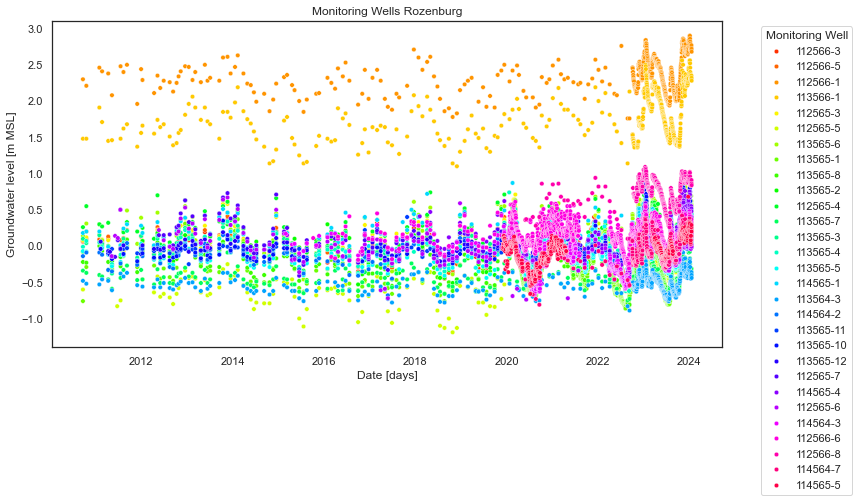
\includegraphics[width=0.80\linewidth]{rozscatter.png}
    \caption{Overview of observed data by manual measurements and data loggers for all 29 monitoring wells in Rozenburg.}
\end{figure}\\

\subsection{Pastas Time Series Modeling}
The bar plot displays the recharge rates in m/day over a period from 2010 to 2024. The x-axis represents the time period from 2010-2024 with the dates labeled on the x-axis. The y-axis quantifies the recharge rate, with values ranging from 0 to a maximum of 0.07 m/day. The bars shows the variability in recharge rates over time, where some years experience peaks in recharge (higher recharge rates), which can be due to increased precipitation. As can be seen from figure 5.2, the data is dense, indicating frequent measurements. The pattern of the bars reflects seasonal changes. Lower values are more frequently observed, possibly indicating a baseline level of recharge over the years. Two additional figures (5.3 and 5.4) of the precipitation and potential evaporation are visualized as well. The data of these figures is combined to determine the recharge rate in the municipal area.


\begin{figure}[htbp]
    \centering
    \includegraphics[width=0.80\linewidth]{figures/res roz/Recharge Rdam.png}
    \caption{Recharge [m/day] over a period of 2010-2024. Recharge is based on the variables precipitation minus evaporation. Variables are  measured by KNMI at weather station 344 in Rotterdam, The Netherlands.}
\end{figure}

\begin{figure}[htbp]
    \centering
    % First figure
    \begin{minipage}{0.45\textwidth}
        \centering
        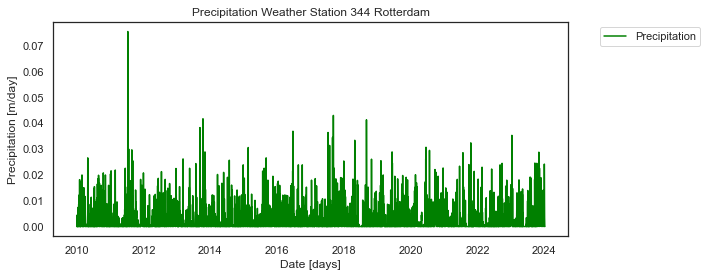
\includegraphics[width=\linewidth]{figures/roz/p.png}
        \caption{Precipitation [m/day] over a period of 2010-2024. Values measured by KNMI at weather station 344 in Rotterdam, The Netherlands.}
        \label{fig:fig1}
    \end{minipage}\hfill
    % Second figure
    \begin{minipage}{0.45\textwidth}
        \centering
        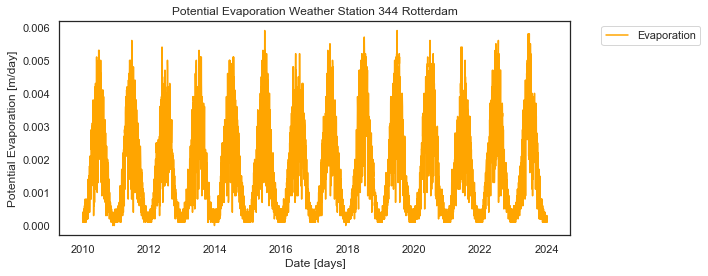
\includegraphics[width=\linewidth]{figures/roz/potevap.png}
        \caption{Potential evaporation [m/day] over a period of 2010-2024. Values measured by KNMI at weather station 344 in Rotterdam, The Netherlands.}
        \label{fig:fig2}
    \end{minipage}
\end{figure}

\subsubsection{Reverse forecasting}
A part of the Pastas package is reverse forecasting or also called backcasting of the observed data. Reversed forecasting takes place for all the unique monitoring wells present in the case study area. For every monitoring well, three figures are created: 1) Reversed backcasting for data loggers; 2) Reversed backcasting for manual measurements; 3) A combination figure of the first 2 figures combined, see figures 5.5-5.7.

\begin{figure}[htbp]
    \centering
    % First figure
    \begin{minipage}{0.32\textwidth}
        \centering
        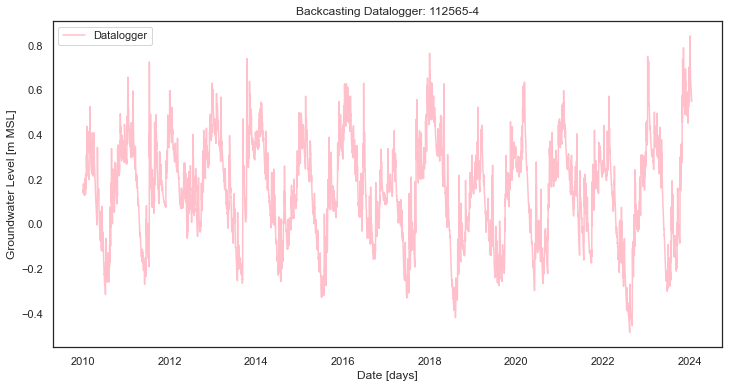
\includegraphics[width=\linewidth]{figures/res roz/backdl1125654.png}
        \caption{Reversed forecasting based on datalogger data for monitoring well 112565-4.}
        \label{fig:112565-3}
    \end{minipage}
    \hfill
    % Second figure
    \begin{minipage}{0.32\textwidth}
        \centering
        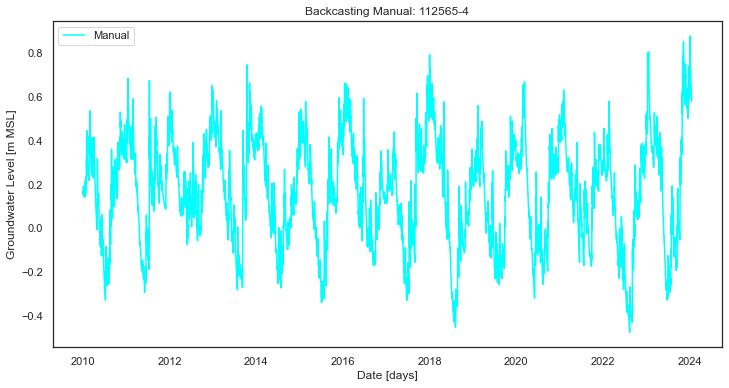
\includegraphics[width=\linewidth]{figures/res roz/backhp1125654.png}
        \caption{Reversed forecasting based on manual measurement data for monitoring well 112565-4.}
        \label{fig:112565-3}
    \end{minipage}
    \hfill
    % Third figure
    \begin{minipage}{0.32\textwidth}
        \centering
        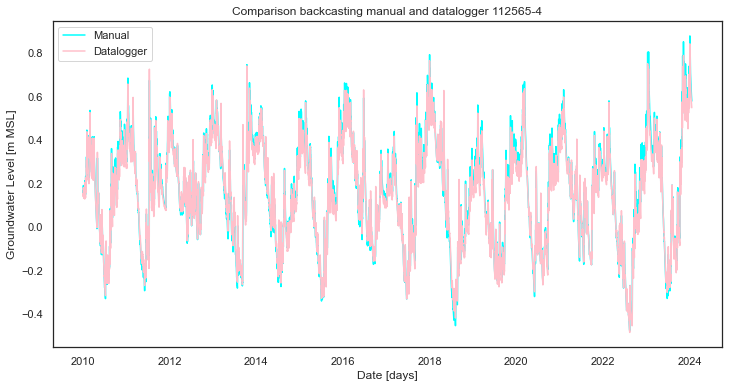
\includegraphics[width=\linewidth]{figures/res roz/comb1125654.png}
        \caption{Reversed forecasting based on manual measurement data and datalogger data for monitoring well 112565-4.}
        \label{fig:112565-3}
    \end{minipage}
\end{figure} \\

\subsubsection{Performance metrics}
The bar plot (fig. 5.8 and 5.9) shows the two metrics RMSE and R2 for all unique monitoring wells. 4 Categories are shown: manual-rmse, manual-rsq, datalogger-rmse, datalogger-rsq. The RMSE seems to be high for some monitoring wells, which could be explained by a high reconstruction error in both of the measurement types. Generally, it looks like the R2 values of the manual measurements are higher than the values of the data loggers. This could suggest that the manual measurements could provide a better fit with the simulated results. The fit of the RMSE and R2 differ for every monitoring well, meaning that there is not a specific pattern that suggests if one of the data groups performs better. An additional bar plot, fig. 5.10, describes the EVP [\%] cross the data set. The EVP is a goodness-of-fit indicator which comparesthe variance of the observed data and the variance of the residual data (Asmuth von et al., 2012). A low EVP indicates that data could be missing in the data set, where the spatial pattern could be a possible reason. A statistical t-test is a follow up, because this can test scientifically and statistically substantiate the difference in performance between the two data groups.  
\newline
Based on the results of the bar plot, the decision was made to execute further statistical tests. A Welch's t-test was carried out, leading to the following results. The Welch's t-test uses an alpha equal to 0.05. 

\begin{figure}[h]
    \centering
    \begin{minipage}{0.48\textwidth}
        \centering
        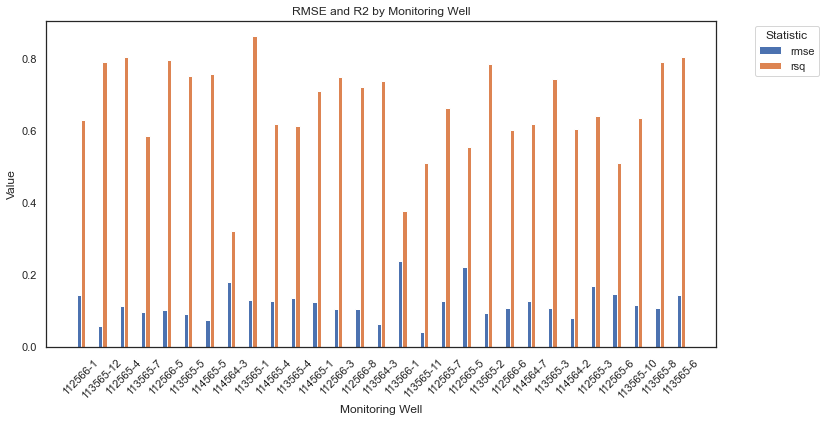
\includegraphics[width=\linewidth]{rmser2roz.png} % Adjust the file name or path as needed.
        \caption{Bar plot of RMSE and R2 for every monitoring well.}
        \label{fig:first-figure}
    \end{minipage}\hfill
    \begin{minipage}{0.48\textwidth}
        \centering
        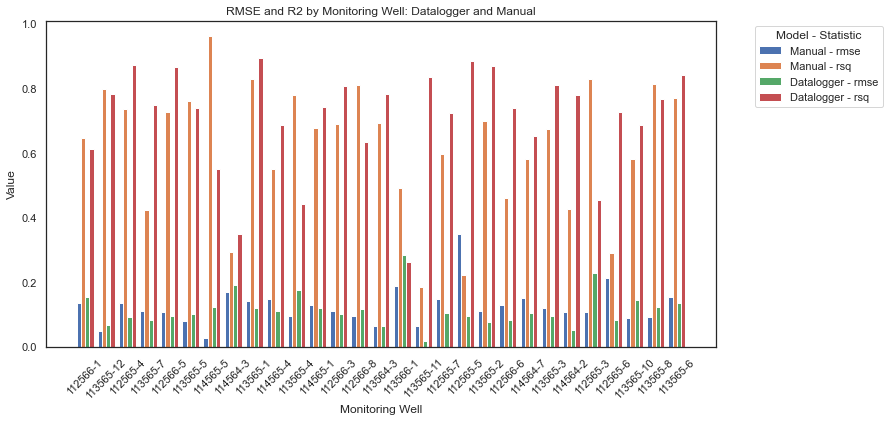
\includegraphics[width=\linewidth]{rmser2roz2.png} % Adjust the file name or path as needed.
        \caption{Bar plot of RMSE and R2 for every monitoring well with a distinction between dataloggers and manual collection.}
        \label{fig:second-figure}
    \end{minipage}
\end{figure}

\begin{figure}[h]
    \centering
    \begin{minipage}{0.48\textwidth}
        \centering
        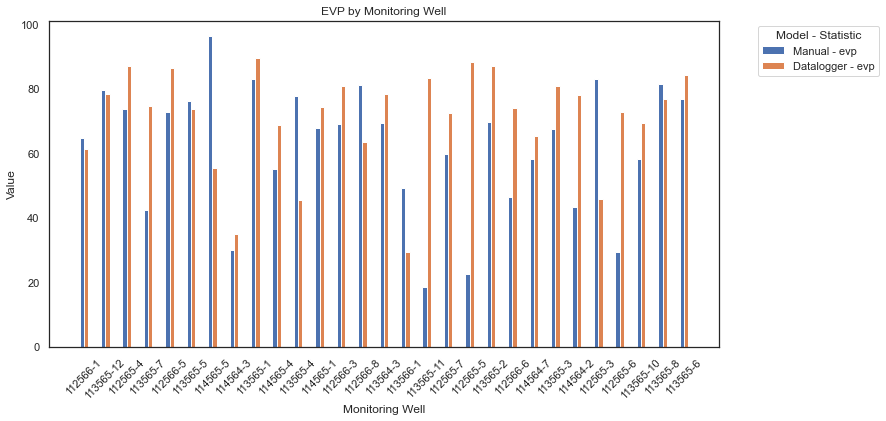
\includegraphics[width=\linewidth]{evproz2.png} % Adjust the file name or path as needed.
        \caption{Bar plot of EVP for every monitoring well.}
        \label{fig:evproz}
    \end{minipage}\hfill
\end{figure}

Figure 5.11 displays the result of the Welch's t-test, based on alpha = 0.5. The results of the performance metrics are labeled as RMSE, R2, and EVP. Each performance metric provides the results of the t-statistic and p-value of the Welch's statistical test. The RMSE (blue section), explains that the t-statistic is negative. This result could indicate that the dataloggers has a lower mean RMSE than the manual collection method. The p-value is higher than alpha = 0.05. A p-value higher than the set alpha explains that no significant difference is present between the dataloggers and manual collection method. The R2 (orange section) explains that the t-statistic is positive, indicating a higher mean R2 for the dataloggers than the manual collection method. The p-value is slightly higher than alpha = 0.05, indicating no significant difference. The last metric is the EVP (green section). The t-statistic of the EVP has a positive value, suggesting that the dataloggers might have a higher mean EVP than the manual collection method. The p-value of 0.065 is very close to 0.05, but resulting in no significant difference. 

\begin{figure}[htbp]
    \centering
    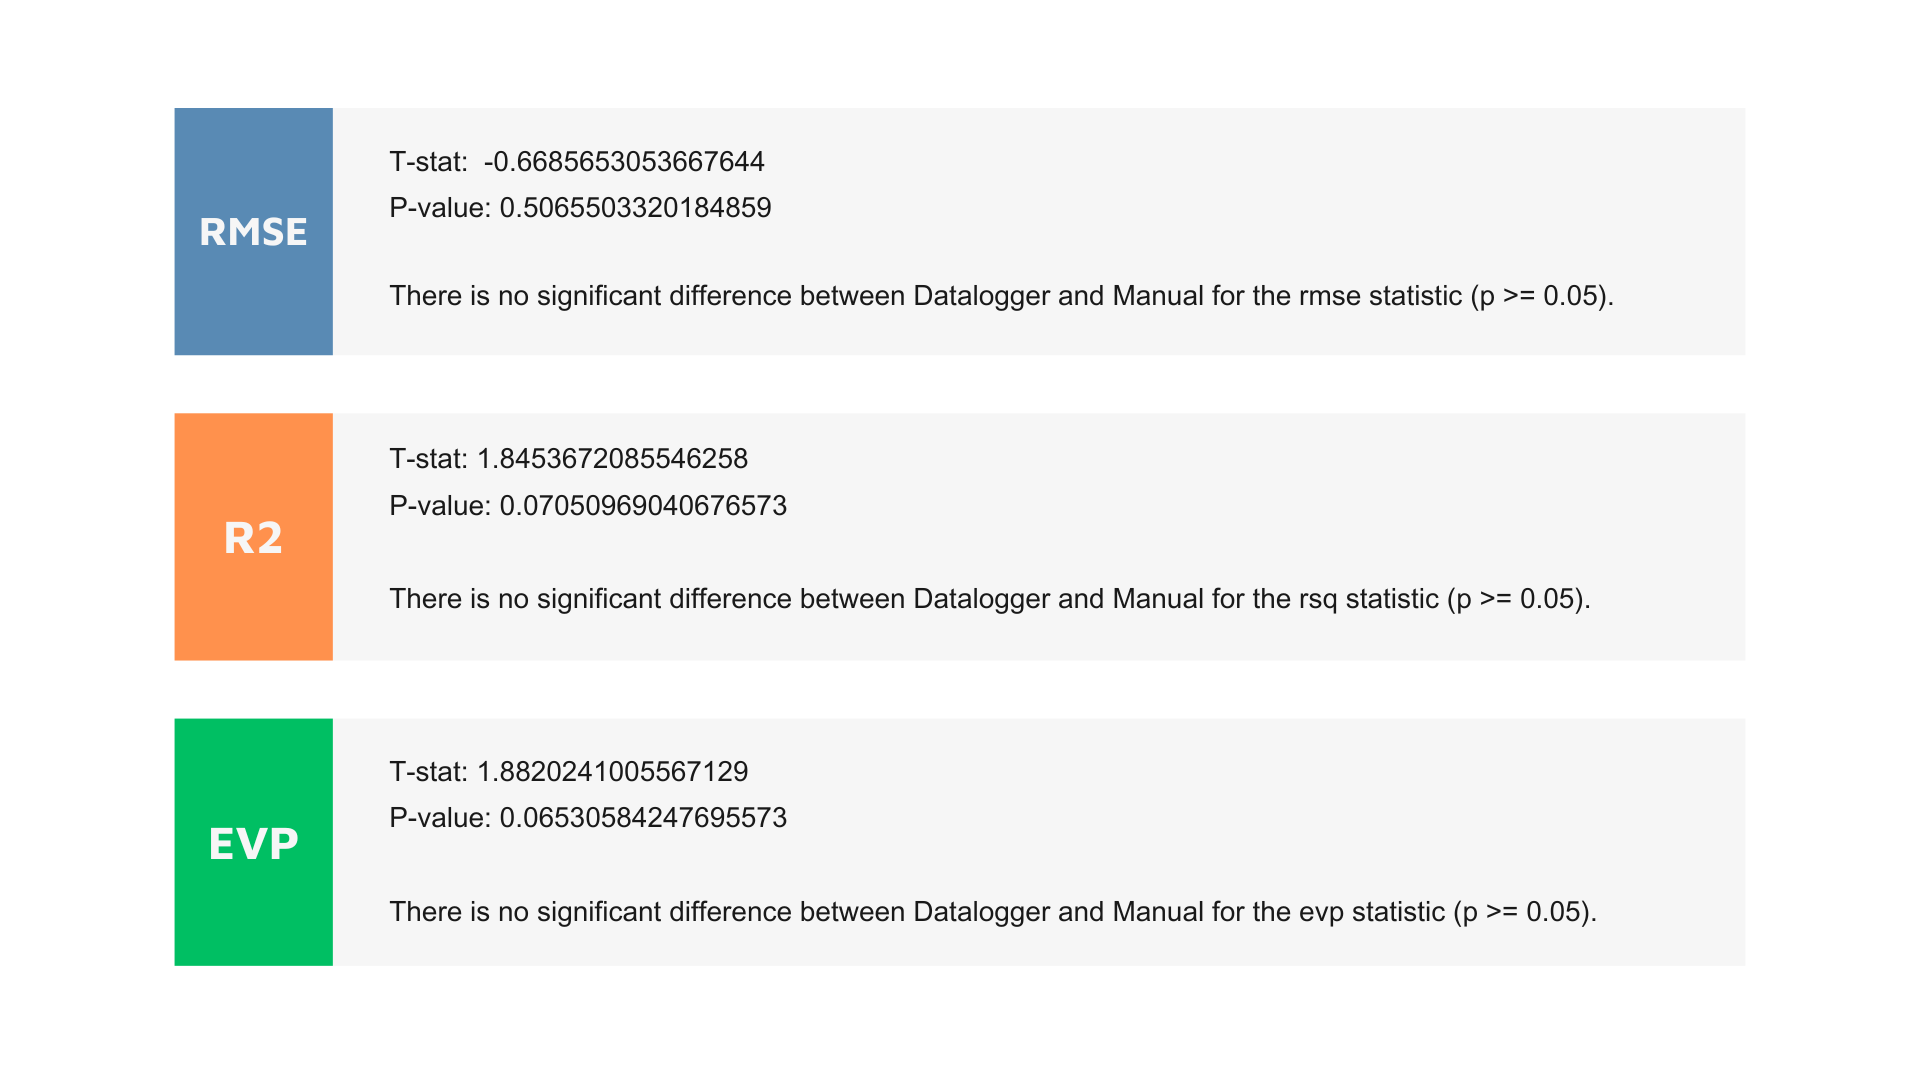
\includegraphics[width=0.80\linewidth]{rozstat.png}
    \caption{Overview of performance metrics of the statistical Welch's test and the difference between dataloggers and manual collection (Author's own contribution).}
\end{figure}

According to the Welch's t-test, no substantial discrepancies were found in the data groups. None of the P-values are below the cut-off of alpha = 0.05. Consequently, it was decided to proceed with the group that is specialized in data loggers. Despite statistical significance, other factors are crucial in environmental sciences. Hence, the datalogger group is chosen, merging observed and simulated data into one dataset and excluding the manual measurements. 

\subsubsection{Creation of new data frame}
The scatter plot below visualizes the observed data logger with the pink scatter and the simulated data of the data logger is visualized by the green scatter. On the x-axis the time period [days] is shown and on the y-axis the groundwater level [m MSL]. Figure 5.12 visualizes only monitoring well 112565-4, the remaining monitoring wells of the neighborhood Rozenburg are available in the appendix and through GitHub.

\begin{figure}[htbp]
    \centering
    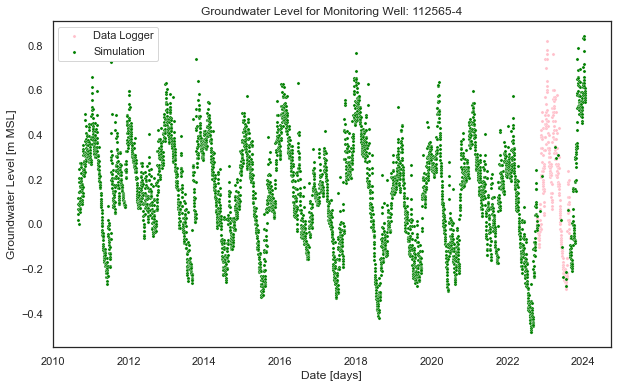
\includegraphics[width=0.80\linewidth]{figures/res roz/sc1125654.png}
    \caption{Scatter plot of merged data frames: observed data by dataloggers and simulation data based on datalogger data for monitoring well 112565-3.}
\end{figure}

\clearpage

\subsection{QR factorization}
Using QR factorization as a foundation, a hierarchical list of the monitoring wells in Rozenburg is created. The optimal reduction percentage is determined and reduction tests can be executed. Resulting in an overview of eliminated monitoring wells and their capability to reconstruct future groundwater levels in the network.

\subsubsection{1D hydrograph data}
Figure 5.13 is a geographical representation (epsg=28992) visualizing the spatial distribution of monitoring wells in the neighborhood "Rozenburg", plotted on a x,y coordinate system. Within the map, a scatter plot with a color scale represents the groundwater level measurements taken at the monitoring wells. The color scale has a range between -0.5 m to +2.0 m MSL. Each monitoring well represents a location as well as the color of monitoring well represents the value on the color scale. In the northwest of the neighborhood, the groundwater level seems to be higher than the groundwater level in the south of the neighborhood. 

\begin{figure}[htbp]
    \centering
    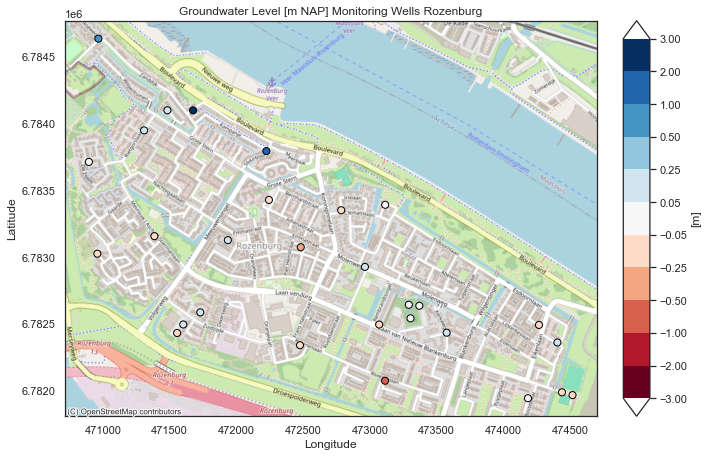
\includegraphics[width=0.80\linewidth]{gwlroz.png}
    \caption{Groundwater level [m MSL] visualized in a geographical map with a color rank that describes the groundwater level observed in the 29 monitoring wells of Rozenburg (Author's own contribution).}
    \label{fig:enter-label}
\end{figure}

\subsubsection{Sampling data}
Preprocessing of the data includes transforming the data frame into an array, implementing both global and local centering methods, and splitting the dataset into an 80/20 ratio training and test set distribution. The result of the preprocessing is as follows, see table 5.1.
\begin{table}[htbp]
\centering
\caption{Summary of sampling data.}
\label{tab:sampling_data}
\begin{tabular}{|l|l|}
\hline
\textbf{Parameter}                           & \textbf{Value}                                \\ \hline
Sampling period                              & 2010-09-02 00:00:00 to 2023-12-31 00:00:00   \\ \hline
Number of samples                            & 4870                                          \\ \hline
Number of features (sensors)                 & 29                                            \\ \hline
Shape of X (samples, sensors)                & (4870, 29)                                    \\ \hline
Min. and max. value                          & -0.8734088406515021 [m] ; 2.857148050691837 [m] \\ \hline
Min. and max. centered value                 & -0.544 [m] 0.732 [m]                         \\ \hline
Min. and max. centered value (exact)         & -0.5436141745216054 [m], 0.7315291423503969 [m] \\ \hline
Mean centered data                           & -0.0 [m]                                     \\ \hline
Train data, Test data                        & 3896 , 974                                   \\ \hline
Train data, Test data (percentage)           & 80\%, 20\%                                  \\ \hline
\end{tabular}
\end{table} 

\subsubsection{Hierarchy of monitoring wells}
A geographical representation (epsg=28992) of data points plotted on a x,y coordinate system is visualized in figure 5.14. The horizontal axis is labeled as longitude and the vertical axis is labeled as latitude. The data points are scattered across the study area within a polygonal boundary that represents the neighborhood "Rozenburg". Each monitoring well monitoring well is color-coded according to the color bar on the right side of the plot. The color indicates the rank of each monitoring well. The color bar has a range between dark blue for the lowest values (0) to a dark red for the highest values (29). The distribution of the color code does not follow a clear pattern within the polygonal boundary. Some clusters of higher or lower ranked monitoring wells are present. Overall, the monitoring wells with additional value are marked blue. They show possibly show flashiness in their data, meaning a high frequency and rapidity in short term changes with strong irregular patterns. According to Ohmer et al. (2022), these monitoring wells indicate strong interaction with surface waters and boundary inflows. As well as a high seasonality and low variability. The monitoring wells that likely do not have additional value to the network are marked red. These wells show low flashiness and high seasonality. The most redundant monitoring wells appear to be located towards the southern edge of the polygonal boundary. At this site, the monitoring wells are clustered, addressing a region of low data variability and flashiness. As well as one single monitoring well in the north of the area. For this monitoring well it does not seem clear why this monitoring wells is redundant, based on other factors as seasonality and flashiness. 

\begin{figure}[h]
    \centering
    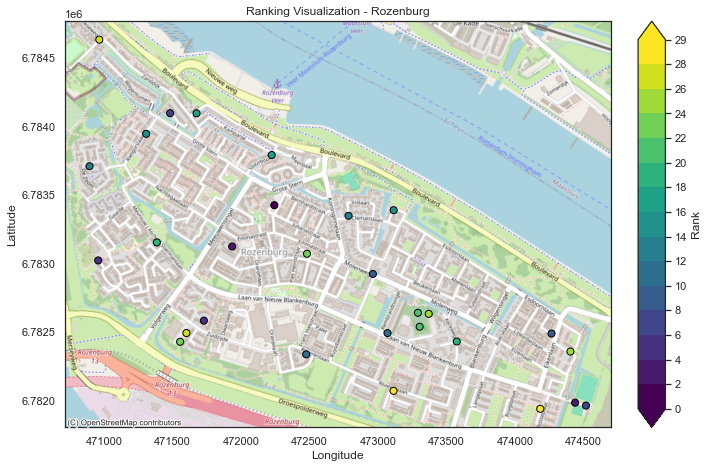
\includegraphics[width=0.80\linewidth]{figures/res roz/opthydro/ranking vis_roz.png}
    \caption{Geographical map visualizing the calculated ranking of all monitoring wells in the neighborhood Rozenburg.}
\end{figure} 

\newpage

\subsubsection{Determining the optimal reduction rate}
In figures 5.15-5.18, the Reconstruction Error of Rozenburg is displayed, plotting the root mean square error (RMSE) in meters on the y-axis against the number of monitoring wells on the x-axis. The line graph shows a decreasing trend in the RMSE as the number of monitoring wells increases, suggesting that more monitoring wells contribute to a lower reconstruction error in the data. In the figures, the orange marked point marks the optimal number of monitoring wells where the reconstruction error reaches the threshold that is indicated by the orange line. The threshold is an acceptable level of RMSE for the reconstruction process. The original groundwater monitoring network of Rozenburg includes 29 monitoring wells.
\newline
In figure 5.15, a reduction of 25\% explains that a number of 21 monitoring wells is the most optimal with a removal of 8 monitoring wells. The RMSE is calculated to determine the optimal number of monitoring wells in the neighborhood. Figure 5.16, demonstrates a trend, based on a reduction rate of 50 \%. The RMSE decreases as more monitoring wells are added to the network. At the point of n=14 on the x-axis, an orange dot is indicated. Beyond this point, the decrease in RMSE slows down, suggesting returns on error reduction after a specific number of monitoring wells is reached. 

\begin{figure}[htbp]
    \centering
    \begin{minipage}[b]{0.48\linewidth}
        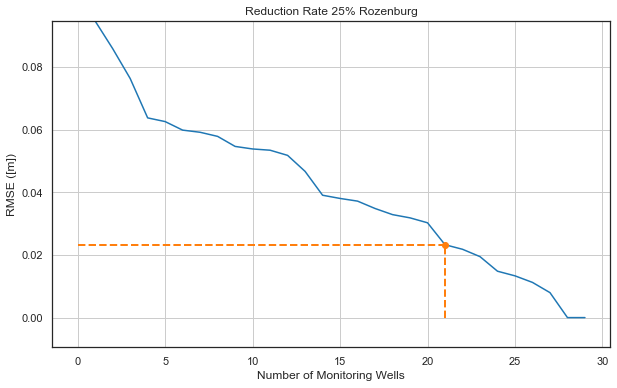
\includegraphics[width=\linewidth]{figures/res roz/25roz.png}
        \caption{Reconstruction error calculated for the neighborhood. The blue line plot visualizes the value of RMSE that differs with the number of monitoring wells. The orange dashed line indicates the optimal number of monitoring wells with the lowest RMSE. RMSE is based on a network reduction of 25 percent.}
        \label{fig:25roz}
    \end{minipage}
    \hfill
    \begin{minipage}[b]{0.48\linewidth}
        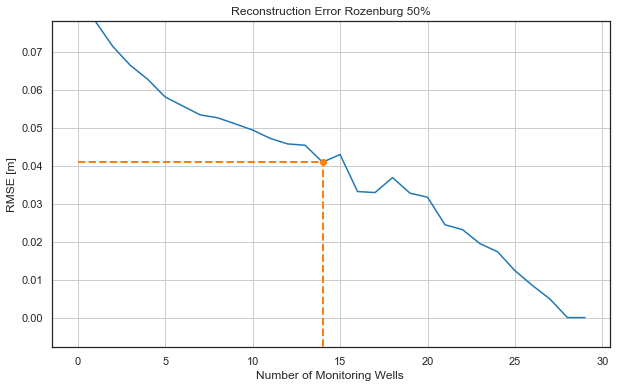
\includegraphics[width=\linewidth]{figures/res roz/roz50.png}
        \caption{Reconstruction error calculated for the neighborhood. The blue line plot visualizes the value of RMSE that differs with the number of monitoring wells. The orange dashed line indicates the optimal number of monitoring wells with the lowest RMSE. RMSE is based on a network reduction of 50 percent.}
        \label{fig:roz50}
    \end{minipage}
\end{figure}

Figure 5.17 displays a trend where the RMSE decreases as the number of monitoring wells increases. The RMSE sharply declines as the monitoring well count approach reaches the point above 10 monitoring wells. This point is marked by the orange dashed line. The line marks the optimal number of monitoring wells where the reconstruction error reaches the threshold value. The threshold value is an acceptable level of RMSE for the reconstruction process. Initially, Rozenburg has 29 monitoring wells. The results of the RMSE explains that only 7 monitoring wells will remain, 22 monitoring wells have to be removed from the local network if a reduction of 75\% is being used in the approach. A reduction rate of 75 percent explains an equilibrium state between the number of monitoring wells and the reconstruction error that is achieved. 
\newline
Continuing with figure 5.18, the Reconstruction Error for a reduction of 90\% is displayed. The figure plots the RMSE in meters on the y-axis against the number of monitoring wells on the x-axis. The line graph shows a sharp decreasing trend in the RMSE as the number of monitoring wells increases. The orange marked point marks the optimal number of monitoring wells where the reconstruction error reaches the threshold that is indicated by the orange line. The threshold is an acceptable level of RMSE for the reconstruction process. Initially, Rozenburg has 29 monitoring wells. The results of the RMSE calculation explains that a number of 2 monitoring wells will remain with this reduction rate, 27 monitoring wells will be removed from the local network. 

\clearpage

\begin{figure}[htbp]
    \centering
    \begin{minipage}{0.48\textwidth}
        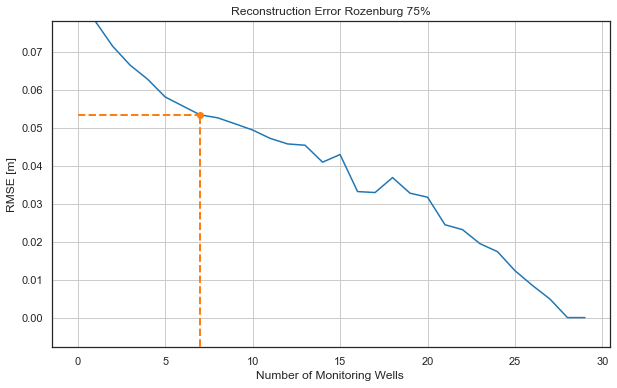
\includegraphics[width=\linewidth]{figures/res roz/roz75.png}
        \caption{Reconstruction error for the neighborhood with network reduction of 75 percent. The blue line shows RMSE variation with the number of monitoring wells, while the orange dashed line indicates the optimal well count for the lowest RMSE.}
        \label{fig:roz75}
    \end{minipage}\hfill
    \begin{minipage}{0.480\textwidth}
        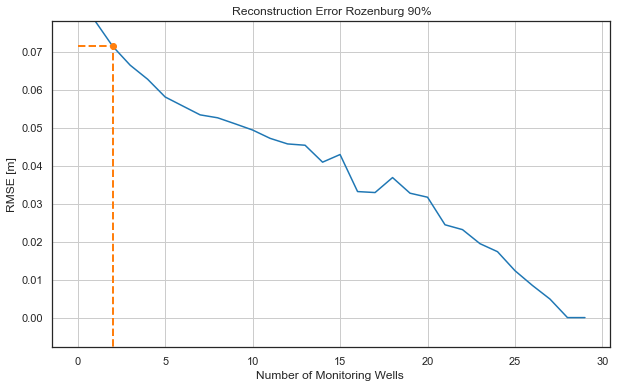
\includegraphics[width=\linewidth]{figures/res roz/roz90.png}
        \caption{Reconstruction error for the neighborhood with network reduction of 90 percent. The blue line shows RMSE variation with the number of monitoring wells, with the orange dashed line showing the optimal number for the lowest RMSE.}
        \label{fig:roz90}
    \end{minipage}
\end{figure}

Based on sensitivity analysis regarding determining the lowest RMSE and MAE as possible for the neighborhood, separate analysis are executed to determine the optimal RMSE and MAE. Further in the analysis, the two performance metrics are combined to determine the lowest RMSE and MAE possible. 

\begin{figure}[htbp]
    \centering
    \begin{minipage}{0.48\textwidth}
        \centering
        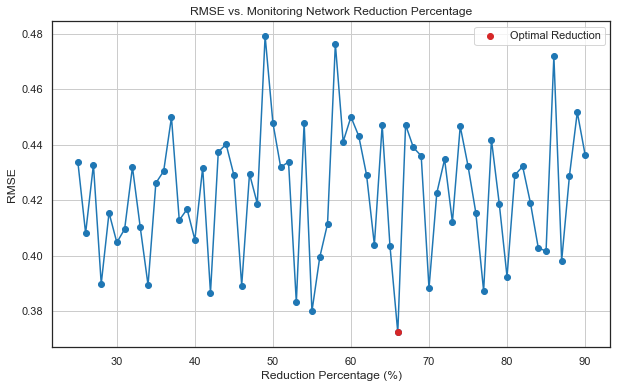
\includegraphics[width=\linewidth]{r2roz.png}
        \caption{Optimal reduction percentage of 66\% based on sensitivity analysis of RMSE.}
        \label{fig:r2roz}
    \end{minipage}\hfill
    \begin{minipage}{0.48\textwidth}
        \centering
        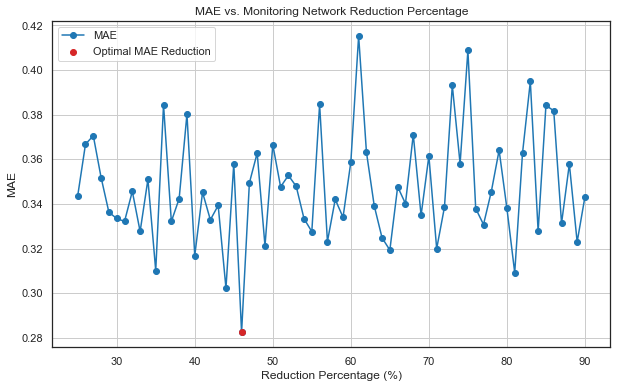
\includegraphics[width=\linewidth]{maeroz.png}
        \caption{Optimal reduction percentage of 46\% based on a sensitivity analysis of MAE.}
        \label{fig:maeroz}
    \end{minipage}
\end{figure}

The normalized RMSE and MAE are combined in figure 5.21. The figure acts as a tool to determine the optimal reduction rate for Rozenburg. The optimal reduction rate lies between 30-40\%. More specifically, a reduction rate of 32\% is achieved with a combined RMSE and MAE of 0.0.

\begin{figure}[htbp]
    \centering
    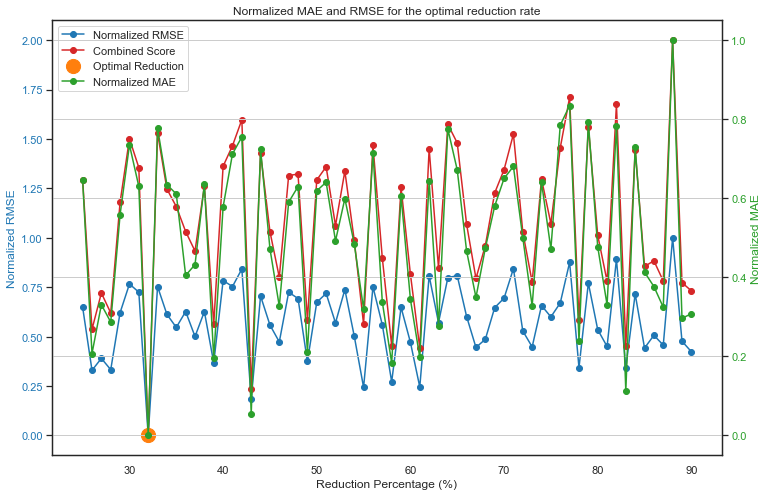
\includegraphics[width=0.80\linewidth]{normroz.png}
    \caption{Visualization of the normalized RMSE and MAE to determine the optimal reduction rate for the GWMN of Rozenburg. The optimal reduction rate lies between 30 and 40\%.}
\end{figure}


\subsubsection{The optimal reduction rate}
According to the sensitivity analysis of the normalized RMSE and MAE, the optimal reduction rate of a monitoring network consisting of 29 monitoring wells counts up to an optimal reduction rate of 32\%. A reduction rate of 32\% implies that the optimal number of monitoring wells in the neighborhood is 19, meaning that 10 monitoring wells are planned to be eliminated, see figure 5.22.

\begin{figure}
    \centering
    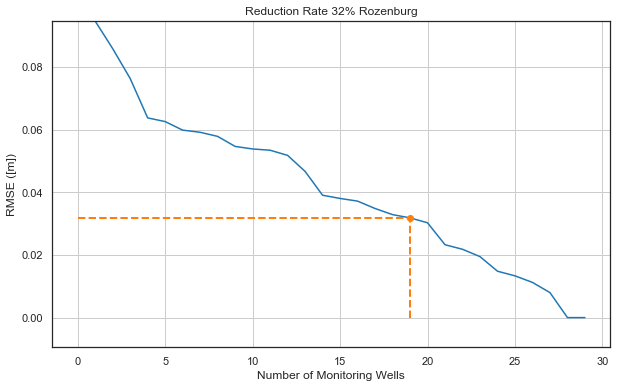
\includegraphics[width=0.8\linewidth]{RRroz32.png}
    \caption{Reconstruction error for the neighborhood with a network reduction of 32\%. The blue line shows RMSE variation with the number of monitoring wells, while the orange dashed line indicates the optimal well count for the lowest RMSE.}
\end{figure}

The reconstruction capability of the eliminated monitoring wells is tested through the creation of hydrographs. The hydrographs include a measured and reconstructed plot. The measured plot (blue line) marks the observed data measured by Gemeente Rotterdam, while the reconstructed plot (red line) marks the reconstructed data based on the observed data and the goodness-of-fit of the model. Performance metrics (MAE, KGE, NSE, R2, RMSE, rBIAS) regarding the goodness-of-fit are available underneath the figure. In figures 5.23-5.32, the hydrographs of the eliminated monitoring wells are shown. 

\begin{figure}[htbp]
    \centering
    % Row 1
    \begin{minipage}{0.48\textwidth}
        \centering
        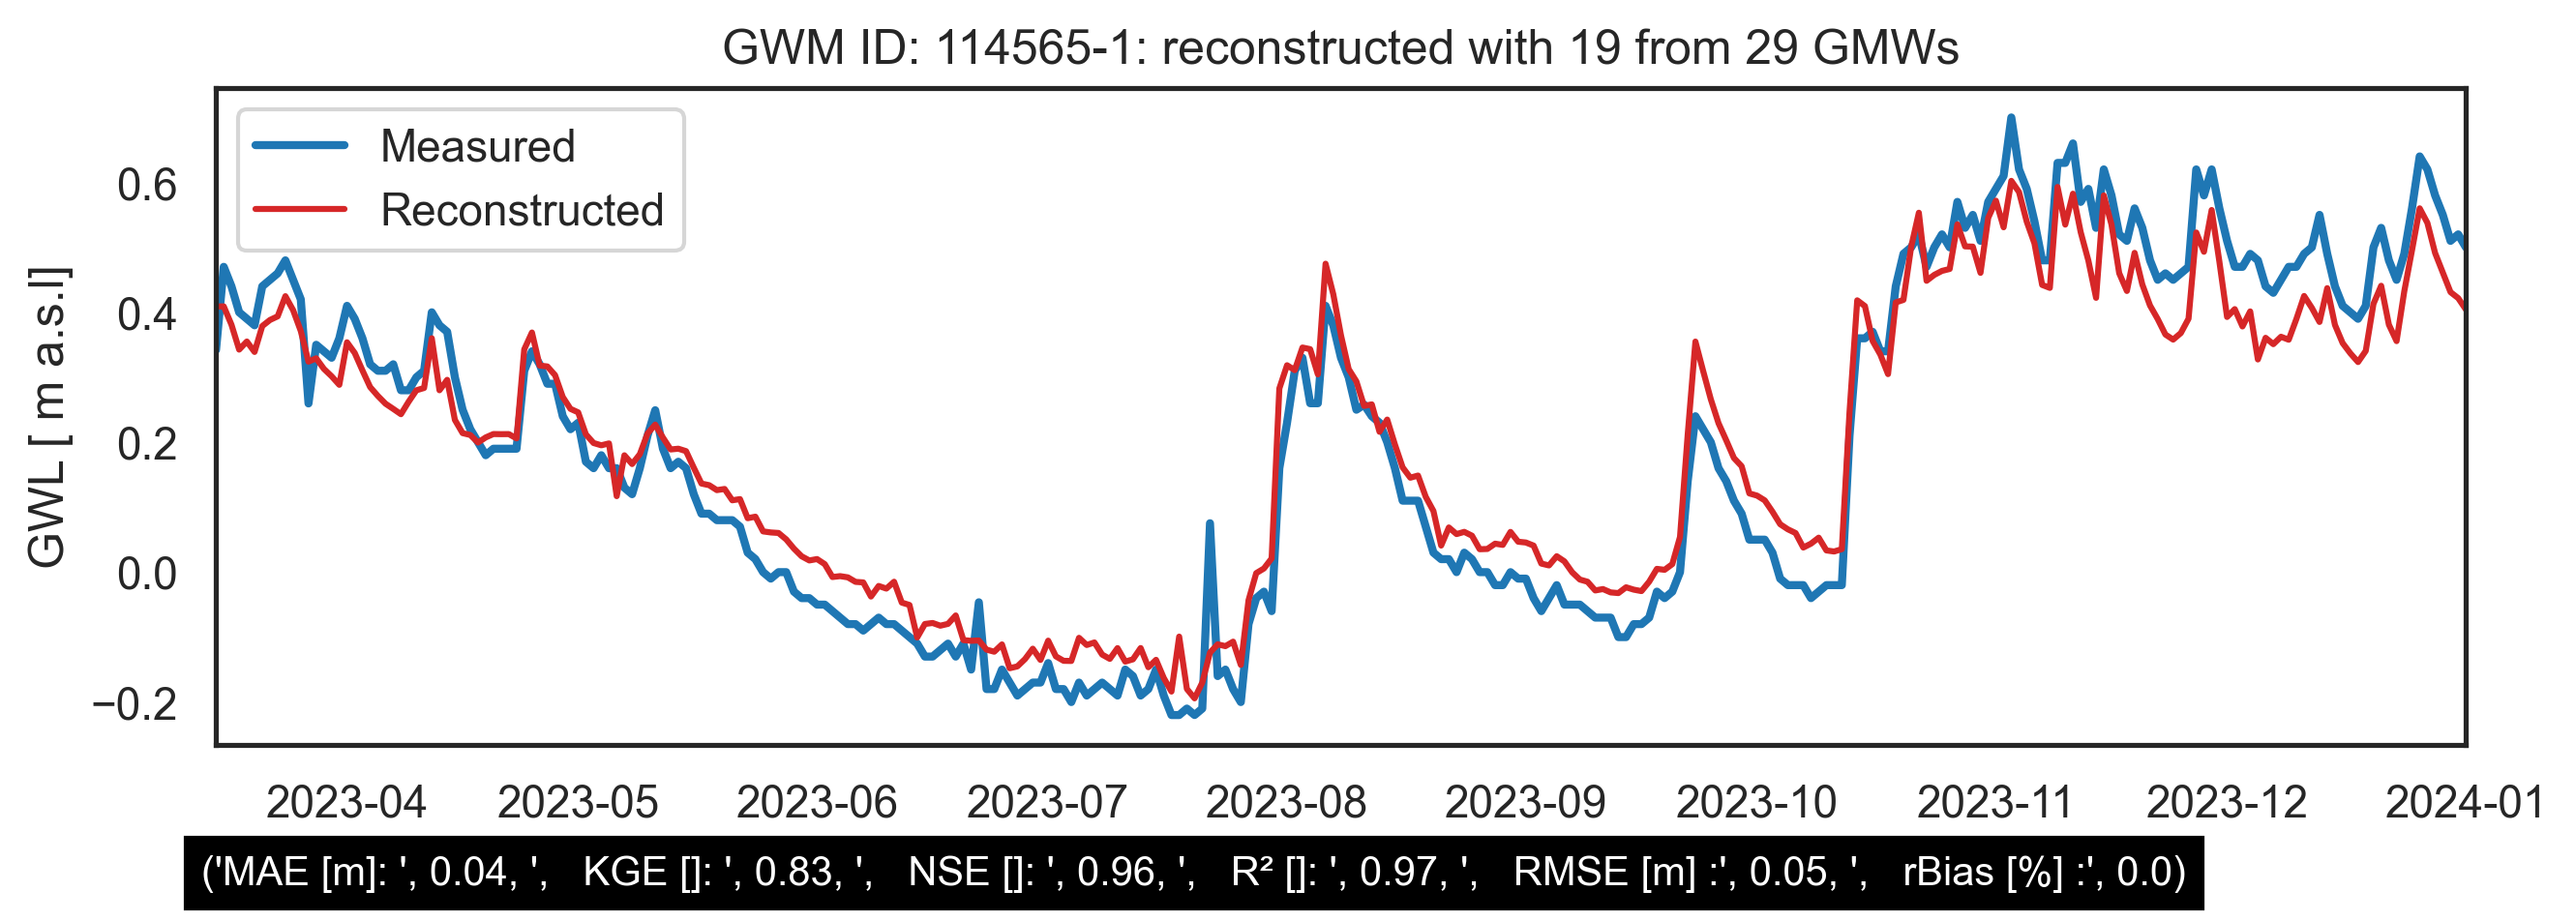
\includegraphics[width=\linewidth]{GWM_reconstructed114565-1.png}
        \caption{Monitoring well: 114565-1.}
        \label{fig:gwm-114565-1}
    \end{minipage}\hfill
    \begin{minipage}{0.48\textwidth}
        \centering
        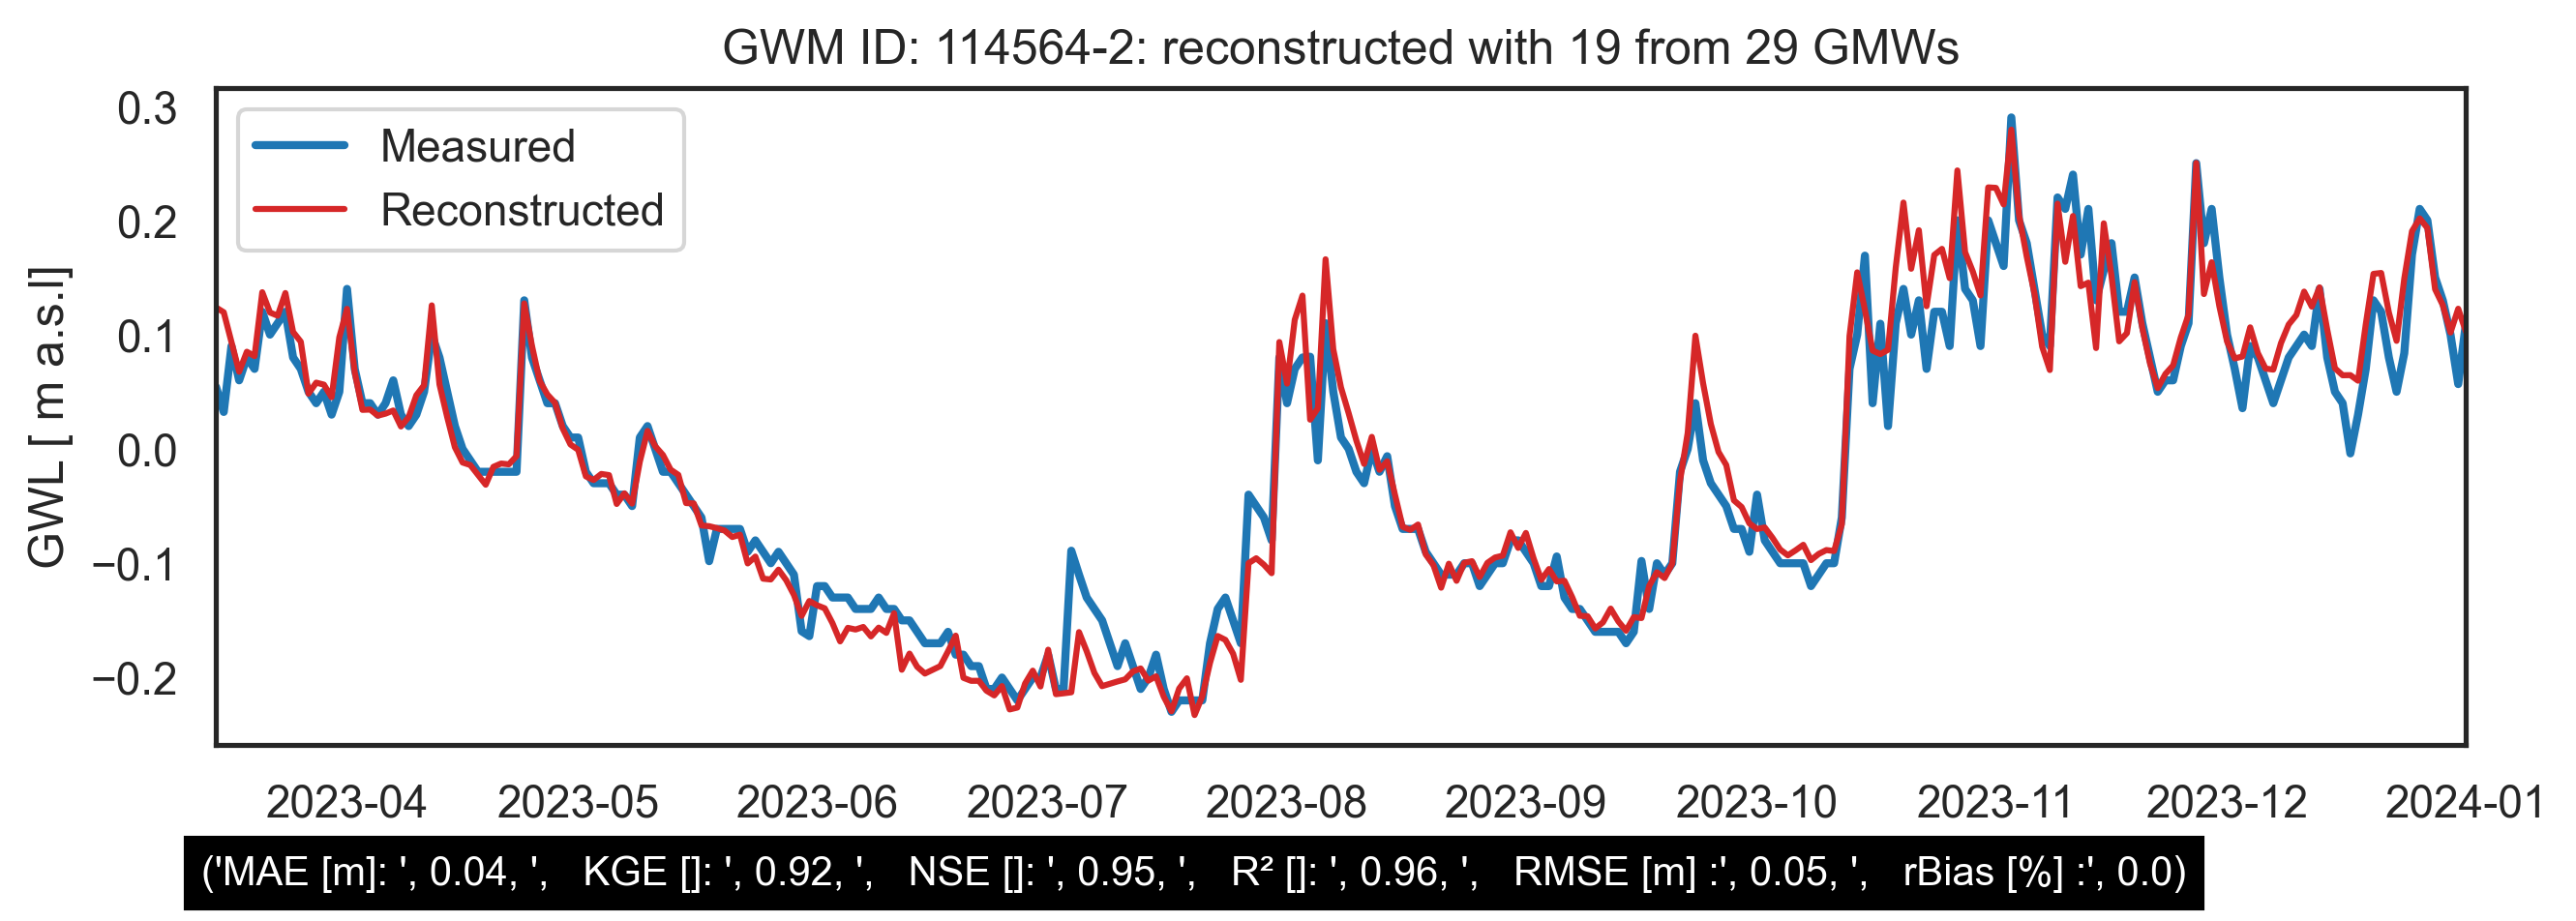
\includegraphics[width=\linewidth]{GWM_reconstructed114564-2.png}
        \caption{Monitoring well: 114564-2.}
        \label{fig:gwm-114564-2}
    \end{minipage}
    
    % Row 2
    \begin{minipage}{0.48\textwidth}
        \centering
        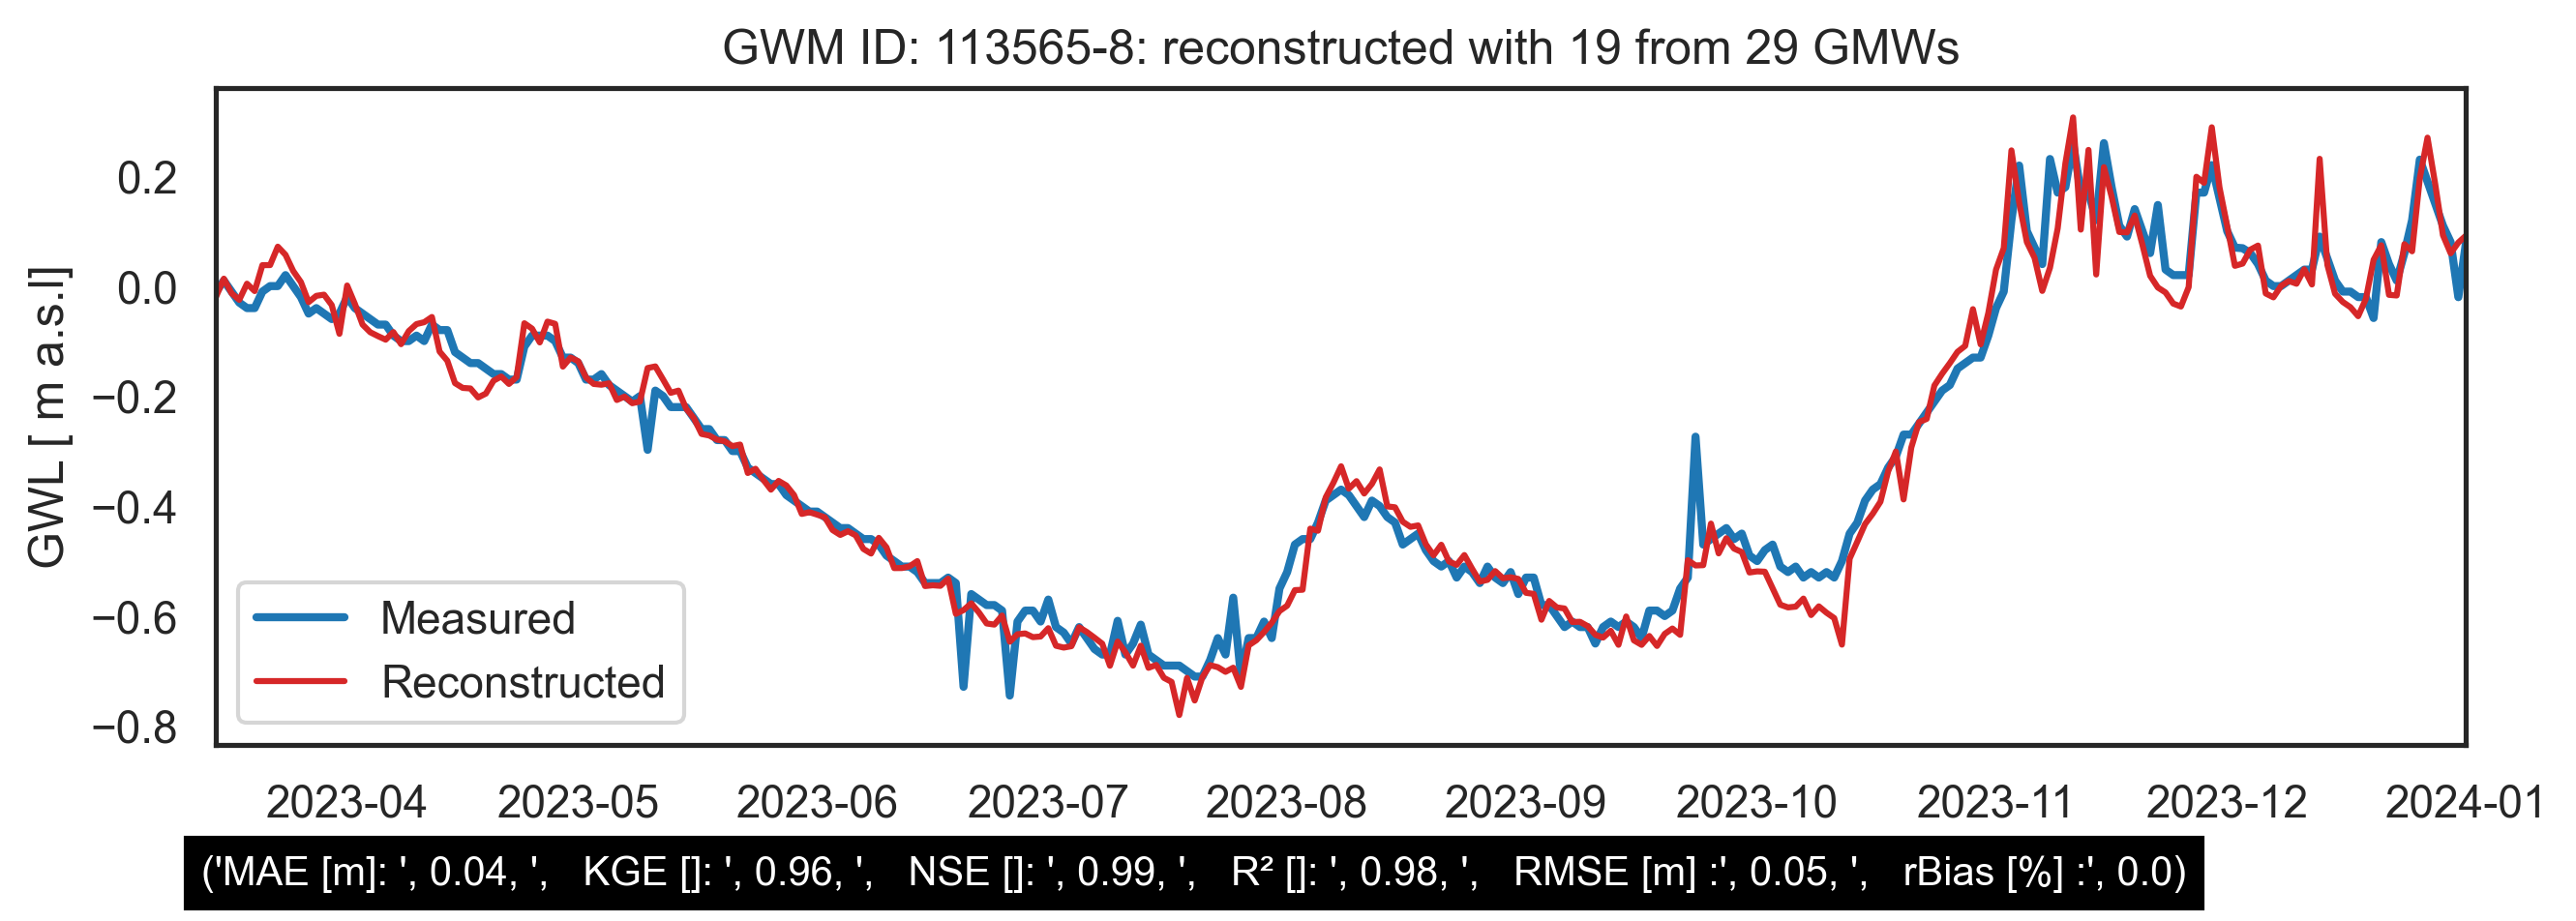
\includegraphics[width=\linewidth]{GWM_reconstructed113565-8.png}
        \caption{Monitoring well: 113565-8.}
        \label{fig:gwm-113565-8}
    \end{minipage}\hfill
    \begin{minipage}{0.48\textwidth}
        \centering
        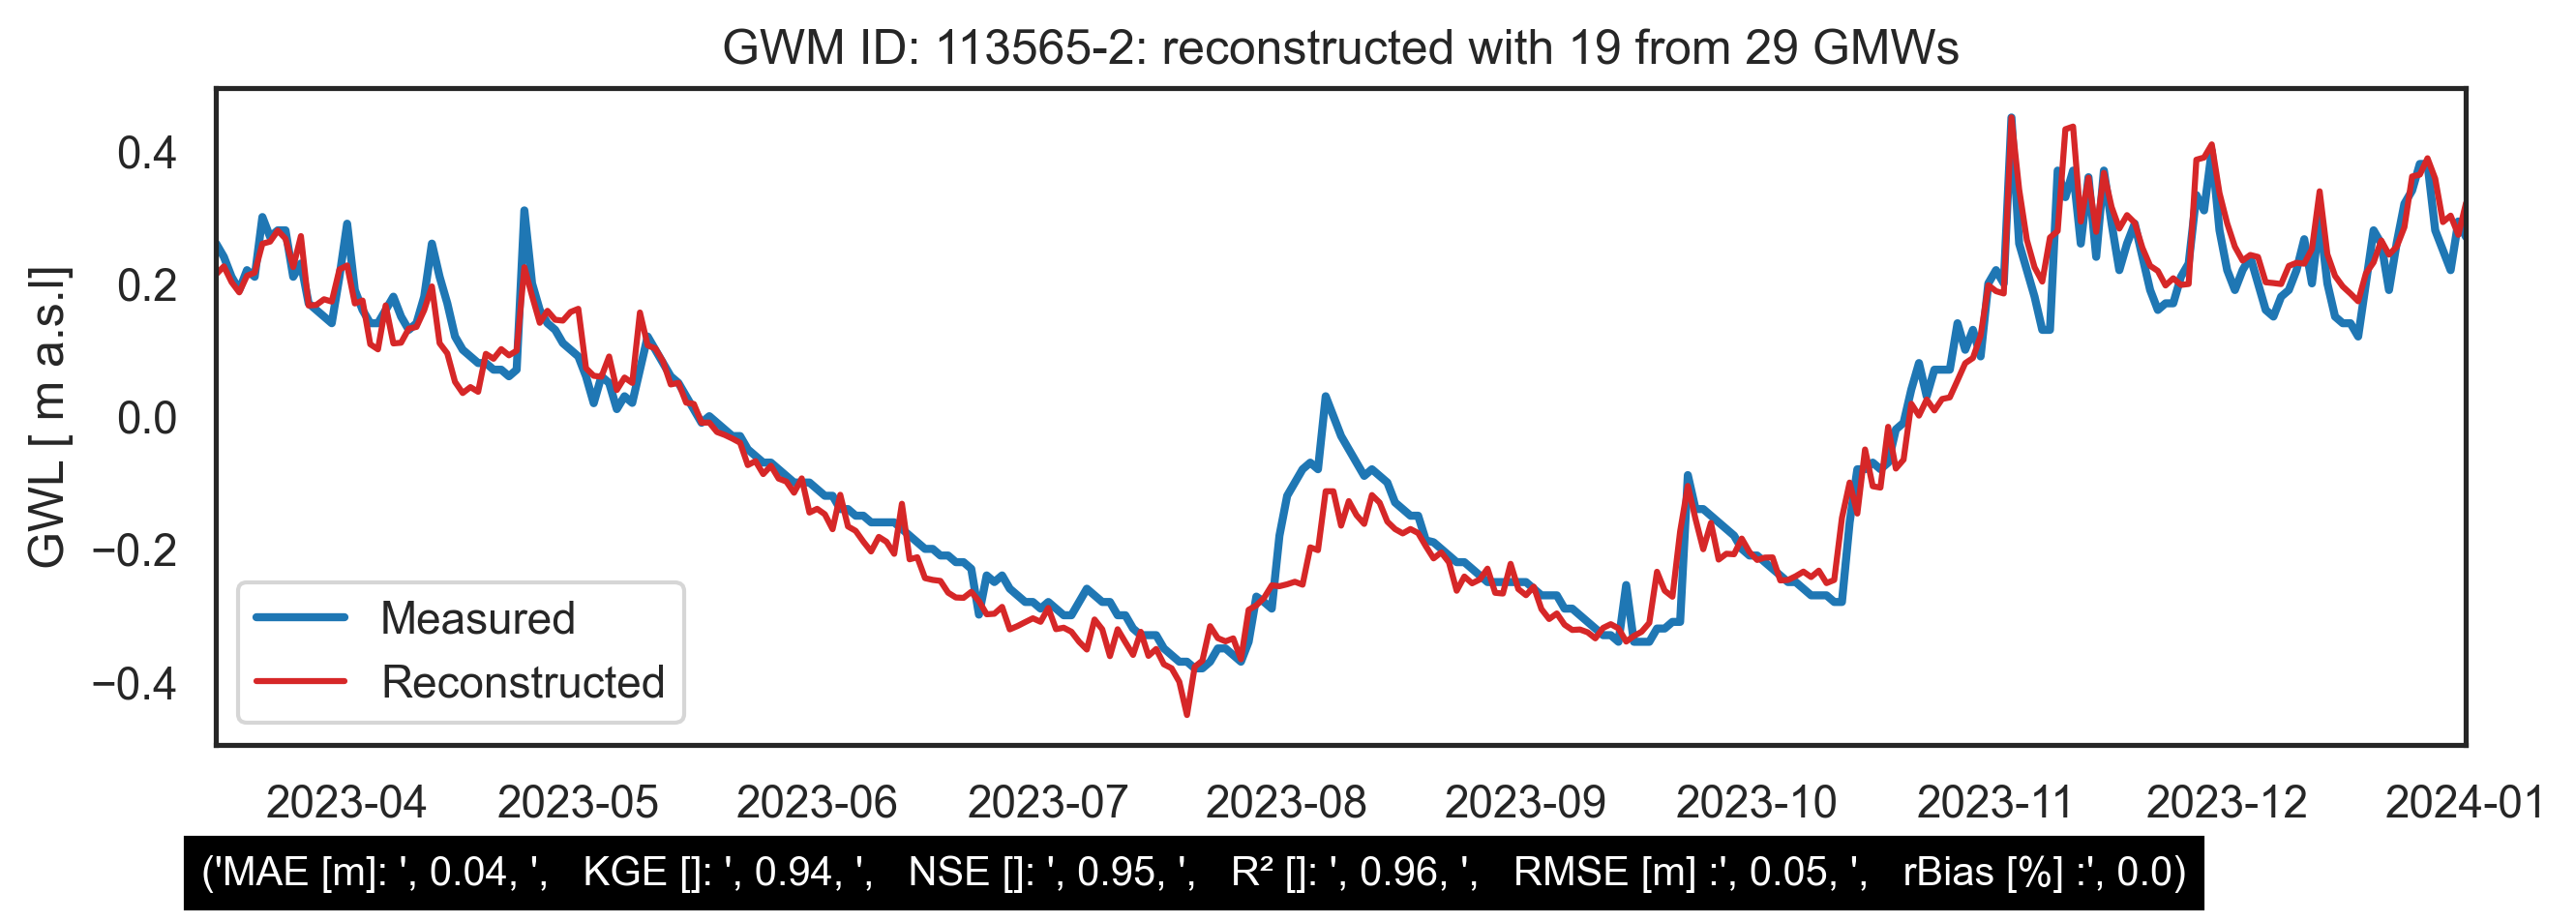
\includegraphics[width=\linewidth]{GWM_reconstructed113565-2.png}
        \caption{Monitoring well: 113565-2.}
        \label{fig:gwm-113565-2}
    \end{minipage}
    
    % Row 3
    \begin{minipage}{0.48\textwidth}
        \centering
        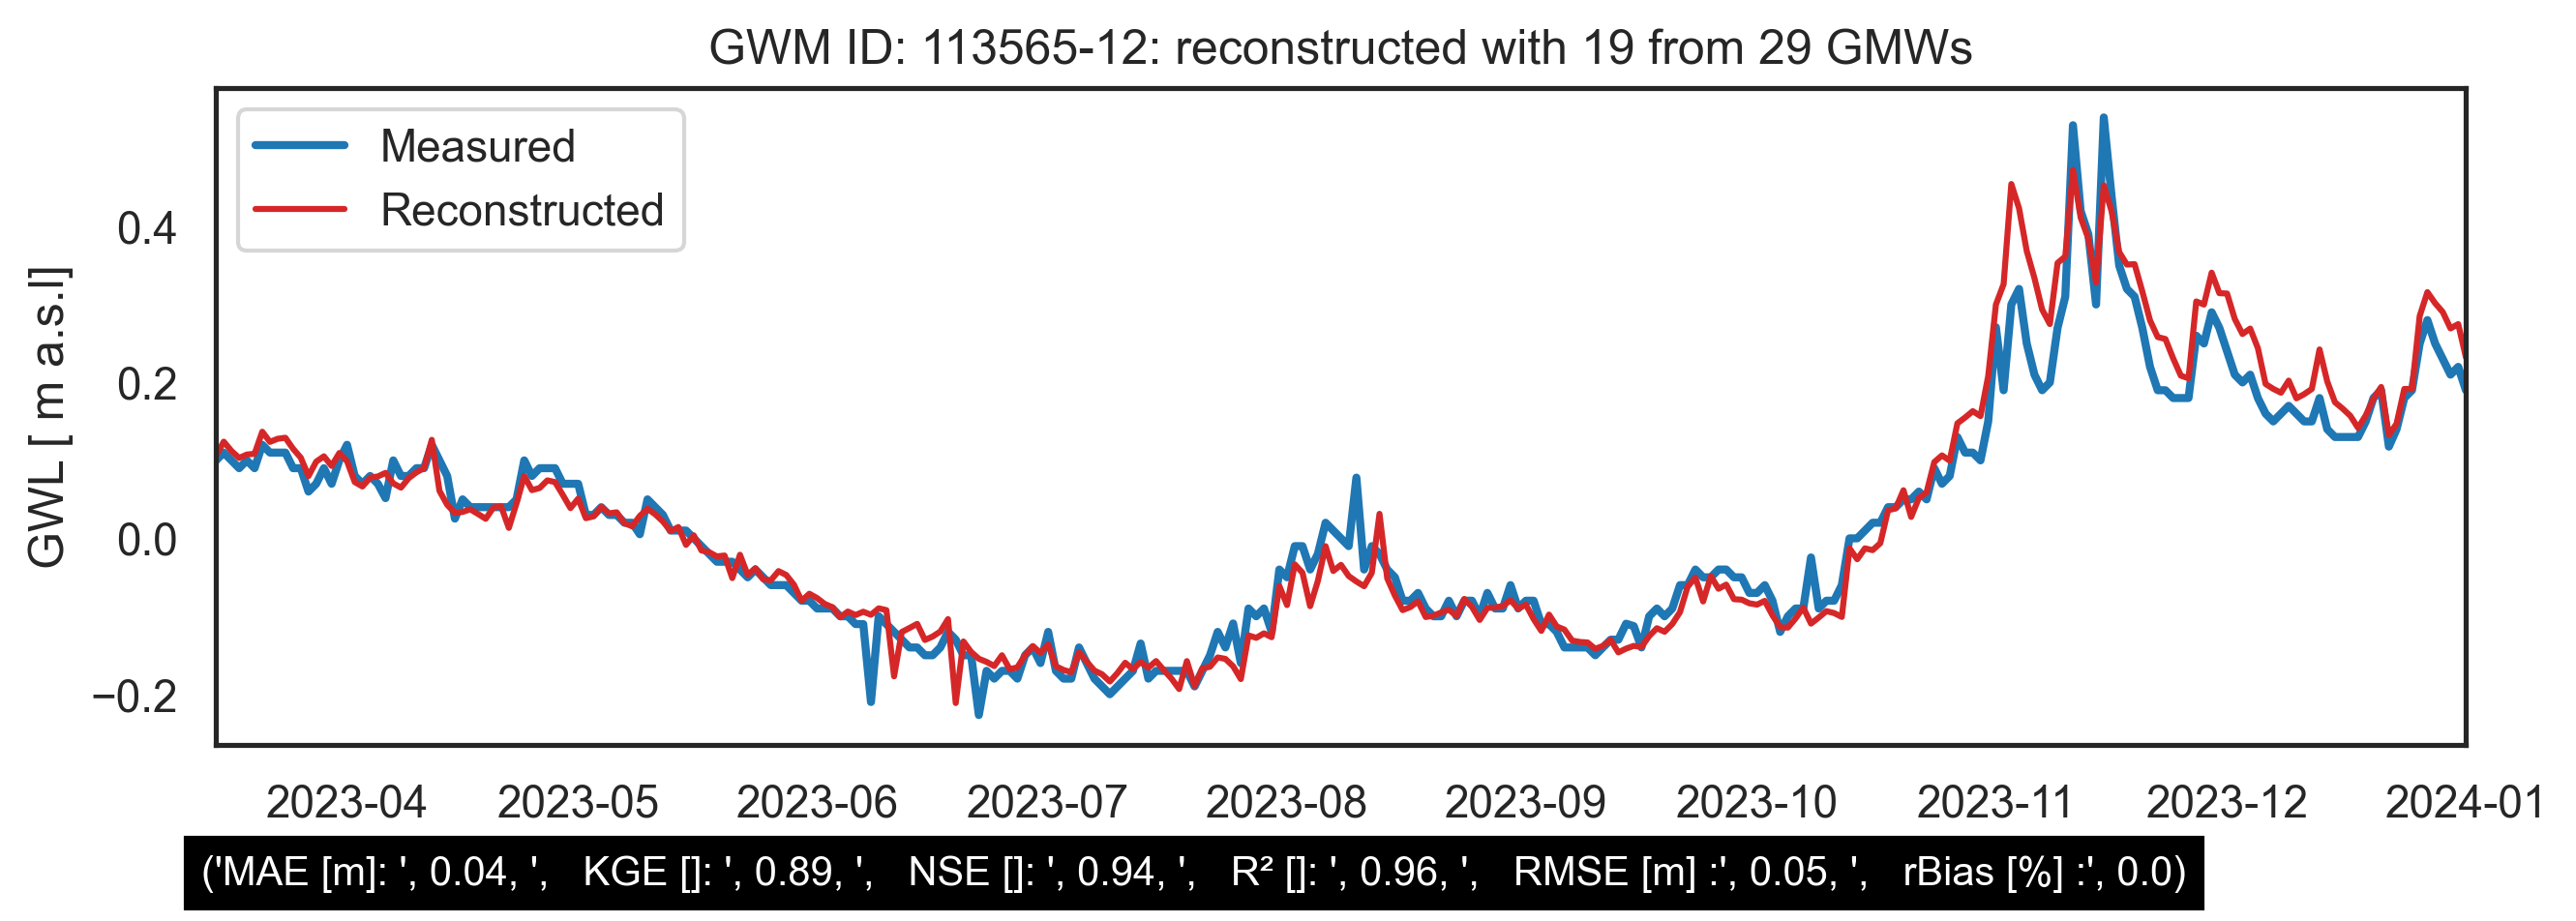
\includegraphics[width=\linewidth]{GWM_reconstructed113565-12.png}
        \caption{Monitoring well: 113565-12.}
        \label{fig:gwm-113565-12}
    \end{minipage}\hfill
    \begin{minipage}{0.48\textwidth}
        \centering
        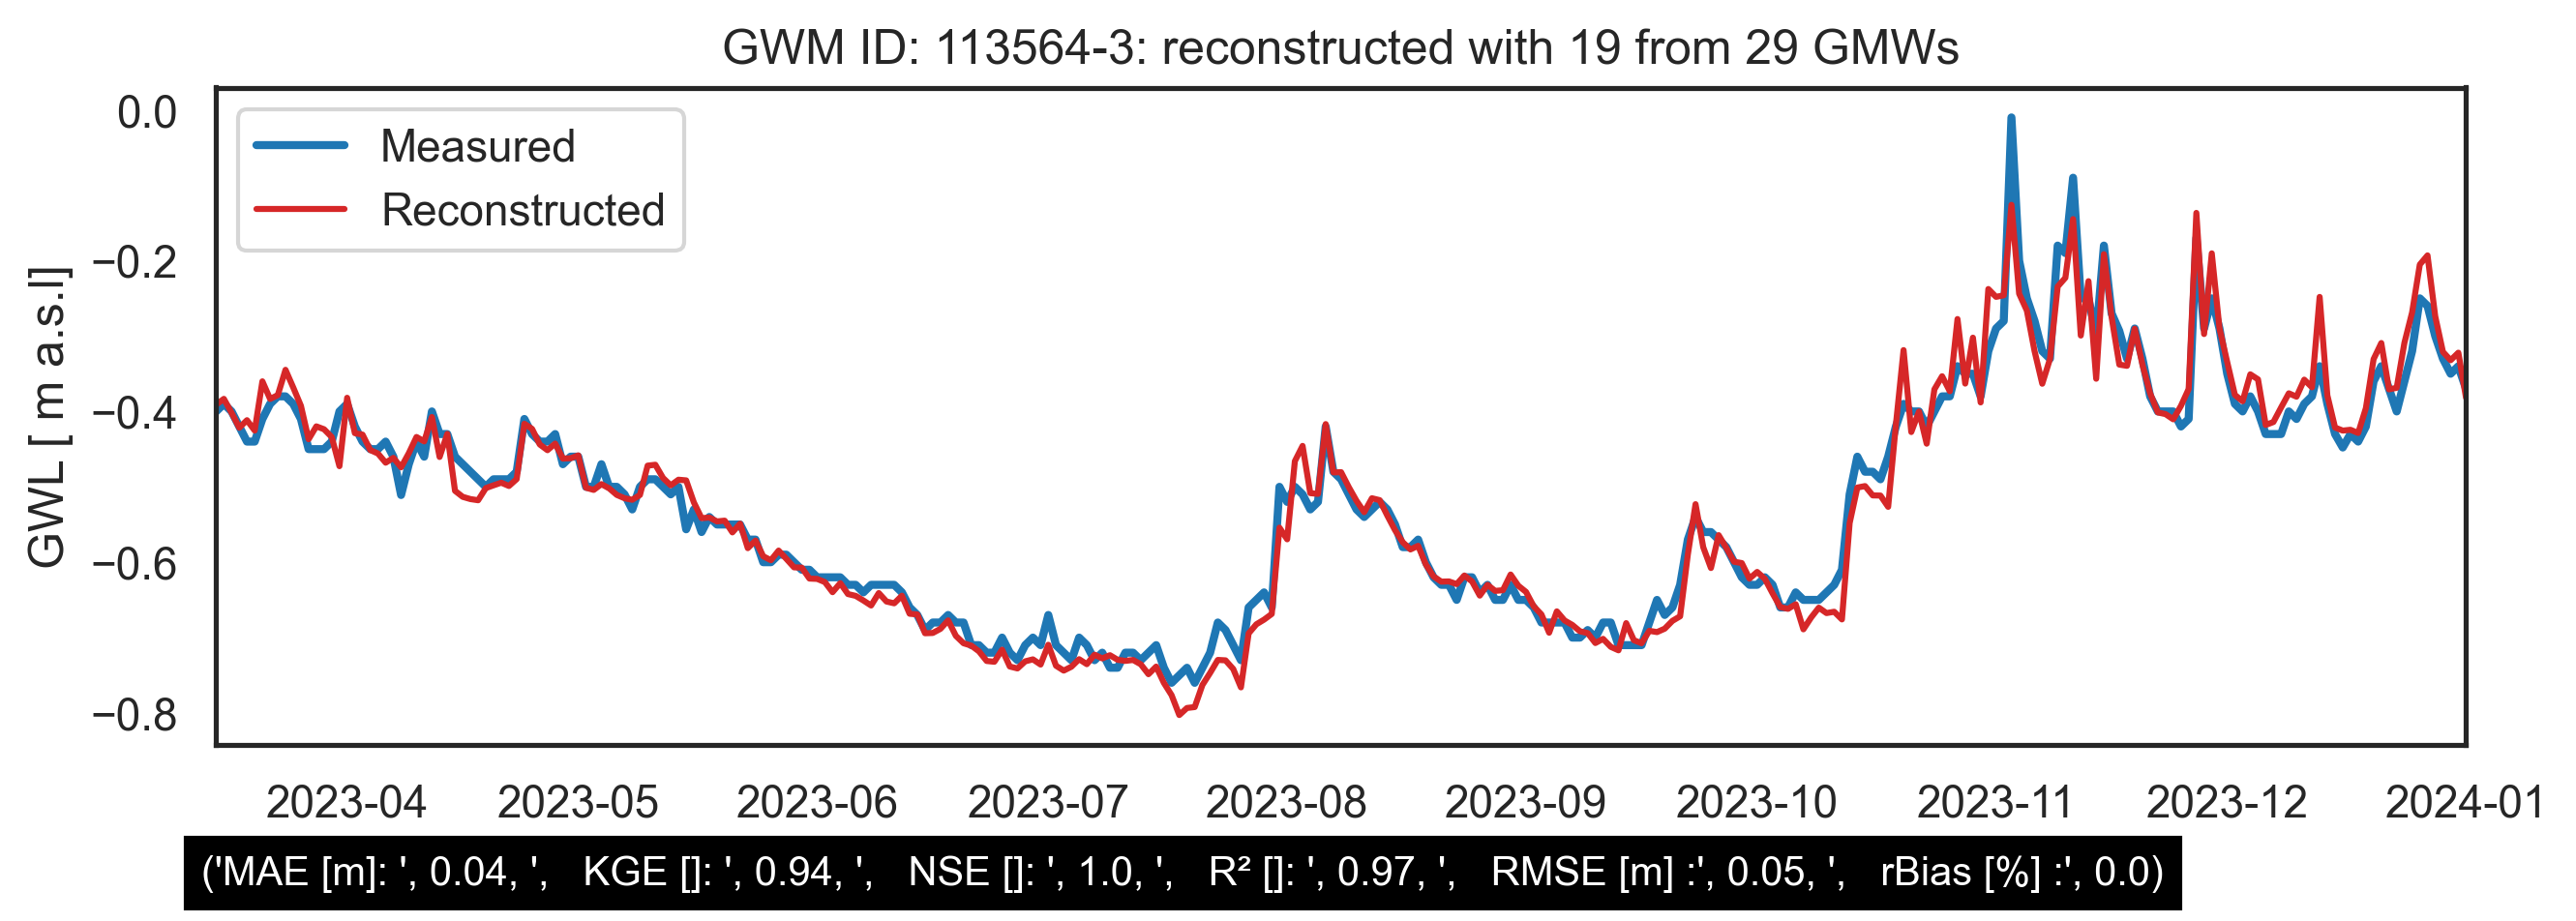
\includegraphics[width=\linewidth]{GWM_reconstructed113564-3.png}
        \caption{Monitoring well: 113564-3.}
        \label{fig:gwm-113564-3}
    \end{minipage}

    % Row 4
    \begin{minipage}{0.48\textwidth}
        \centering
        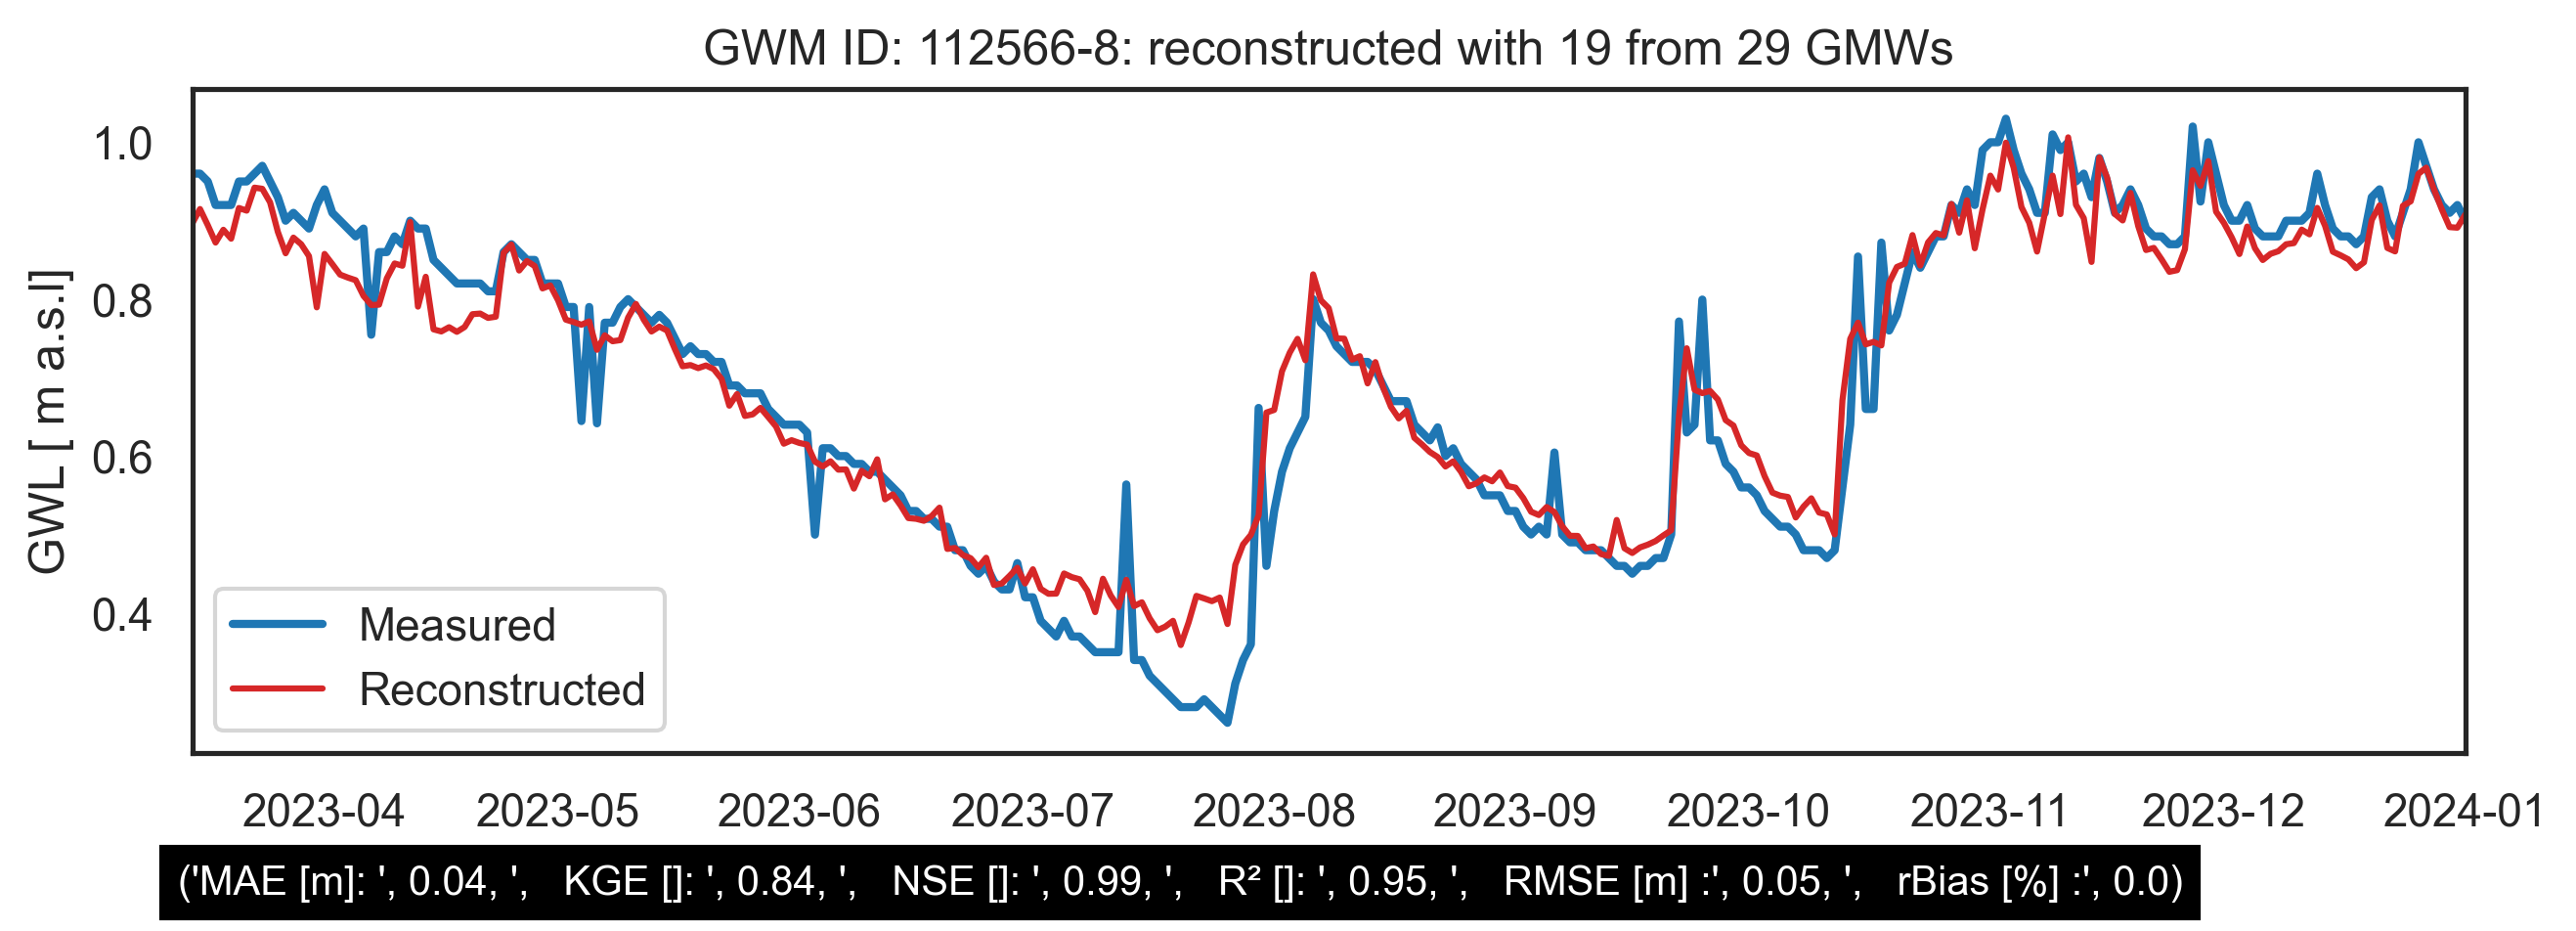
\includegraphics[width=\linewidth]{GWM_reconstructed112566-8.png}
        \caption{Monitoring well: 112566-8.}
        \label{fig:gwm-112566-8}
    \end{minipage}\hfill
    \begin{minipage}{0.48\textwidth}
        \centering
        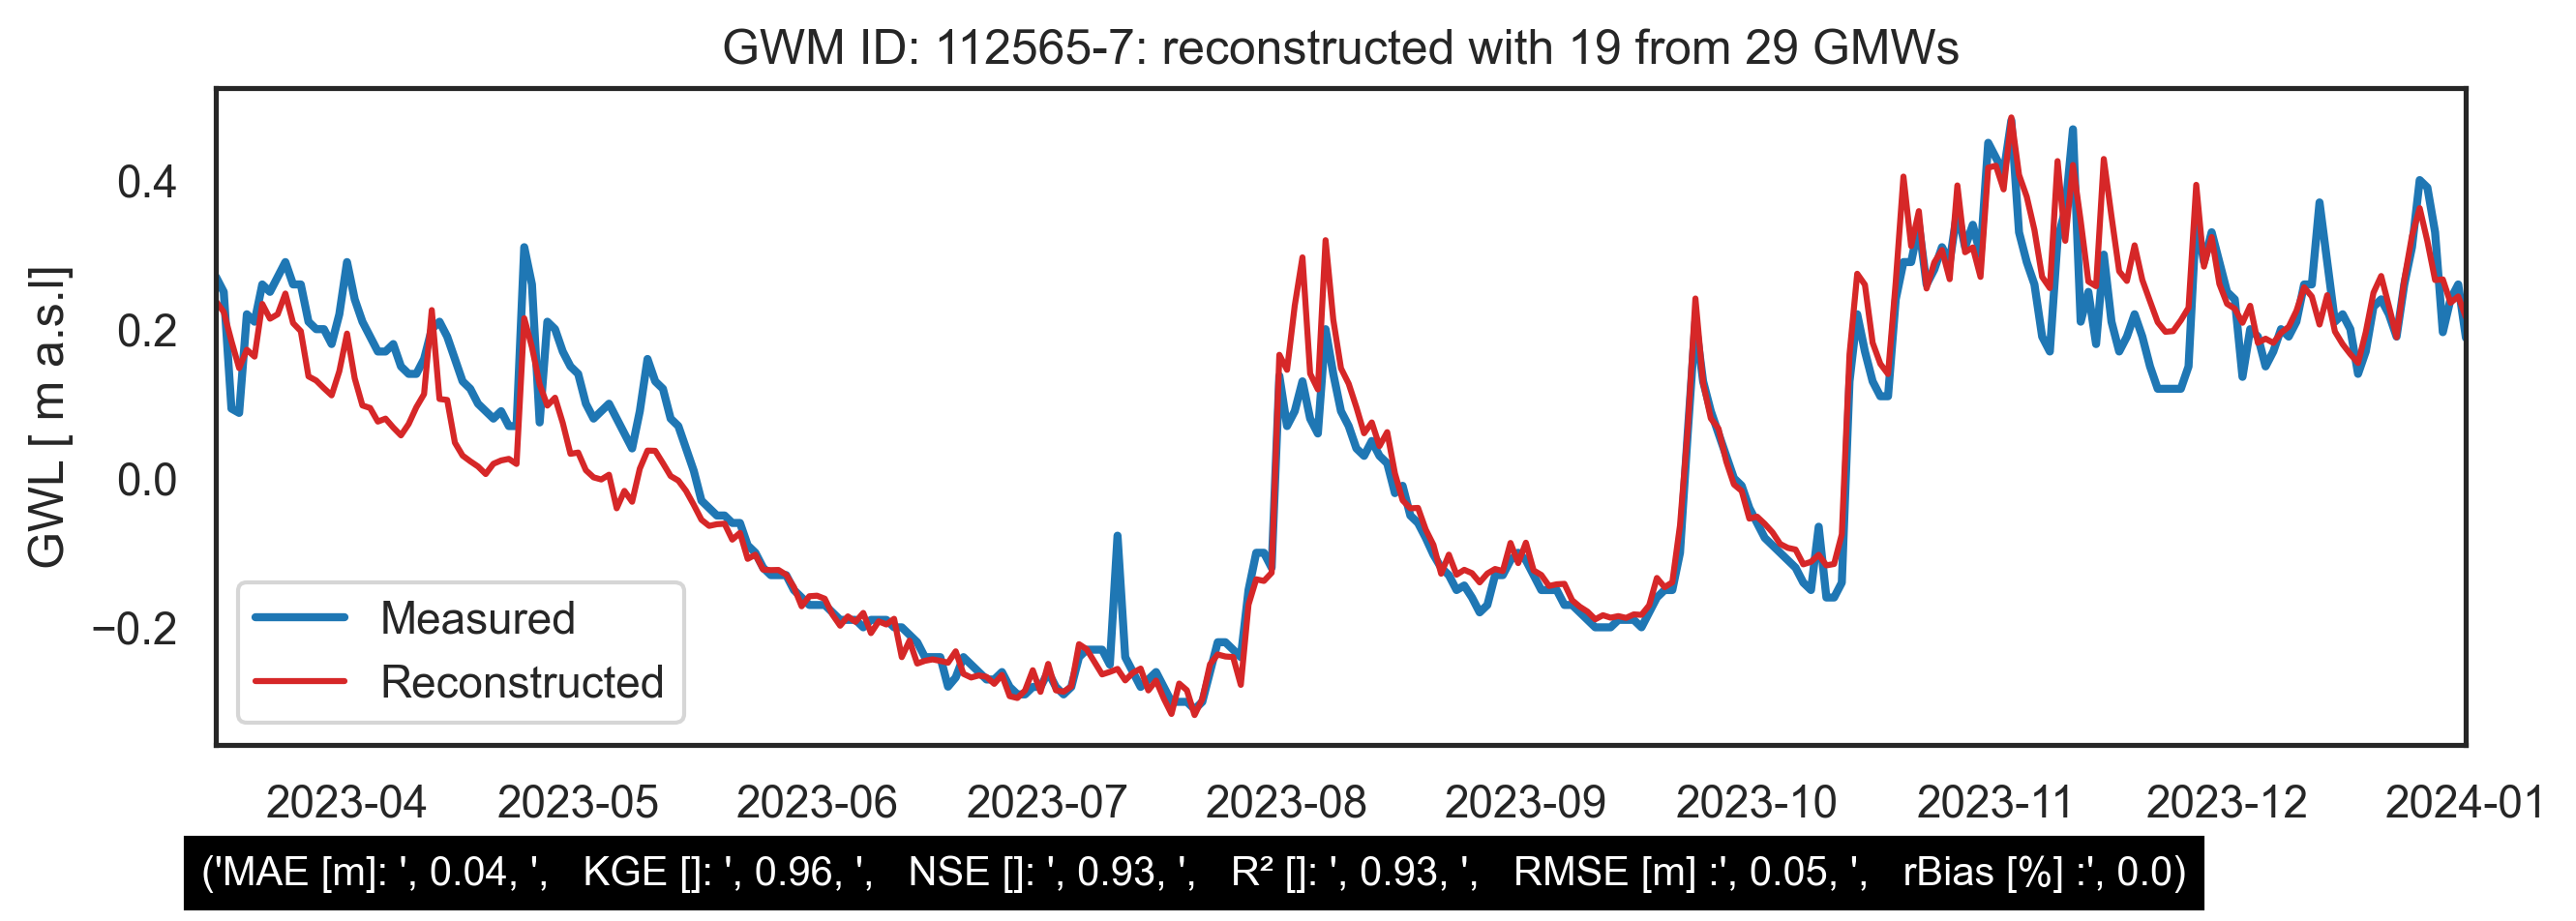
\includegraphics[width=\linewidth]{GWM_reconstructed112565-7.png}
        \caption{Monitoring well: 112565-7.}
        \label{fig:gwm-112565-7}
    \end{minipage}

    % Row 5
    \begin{minipage}{0.48\textwidth}
        \centering
        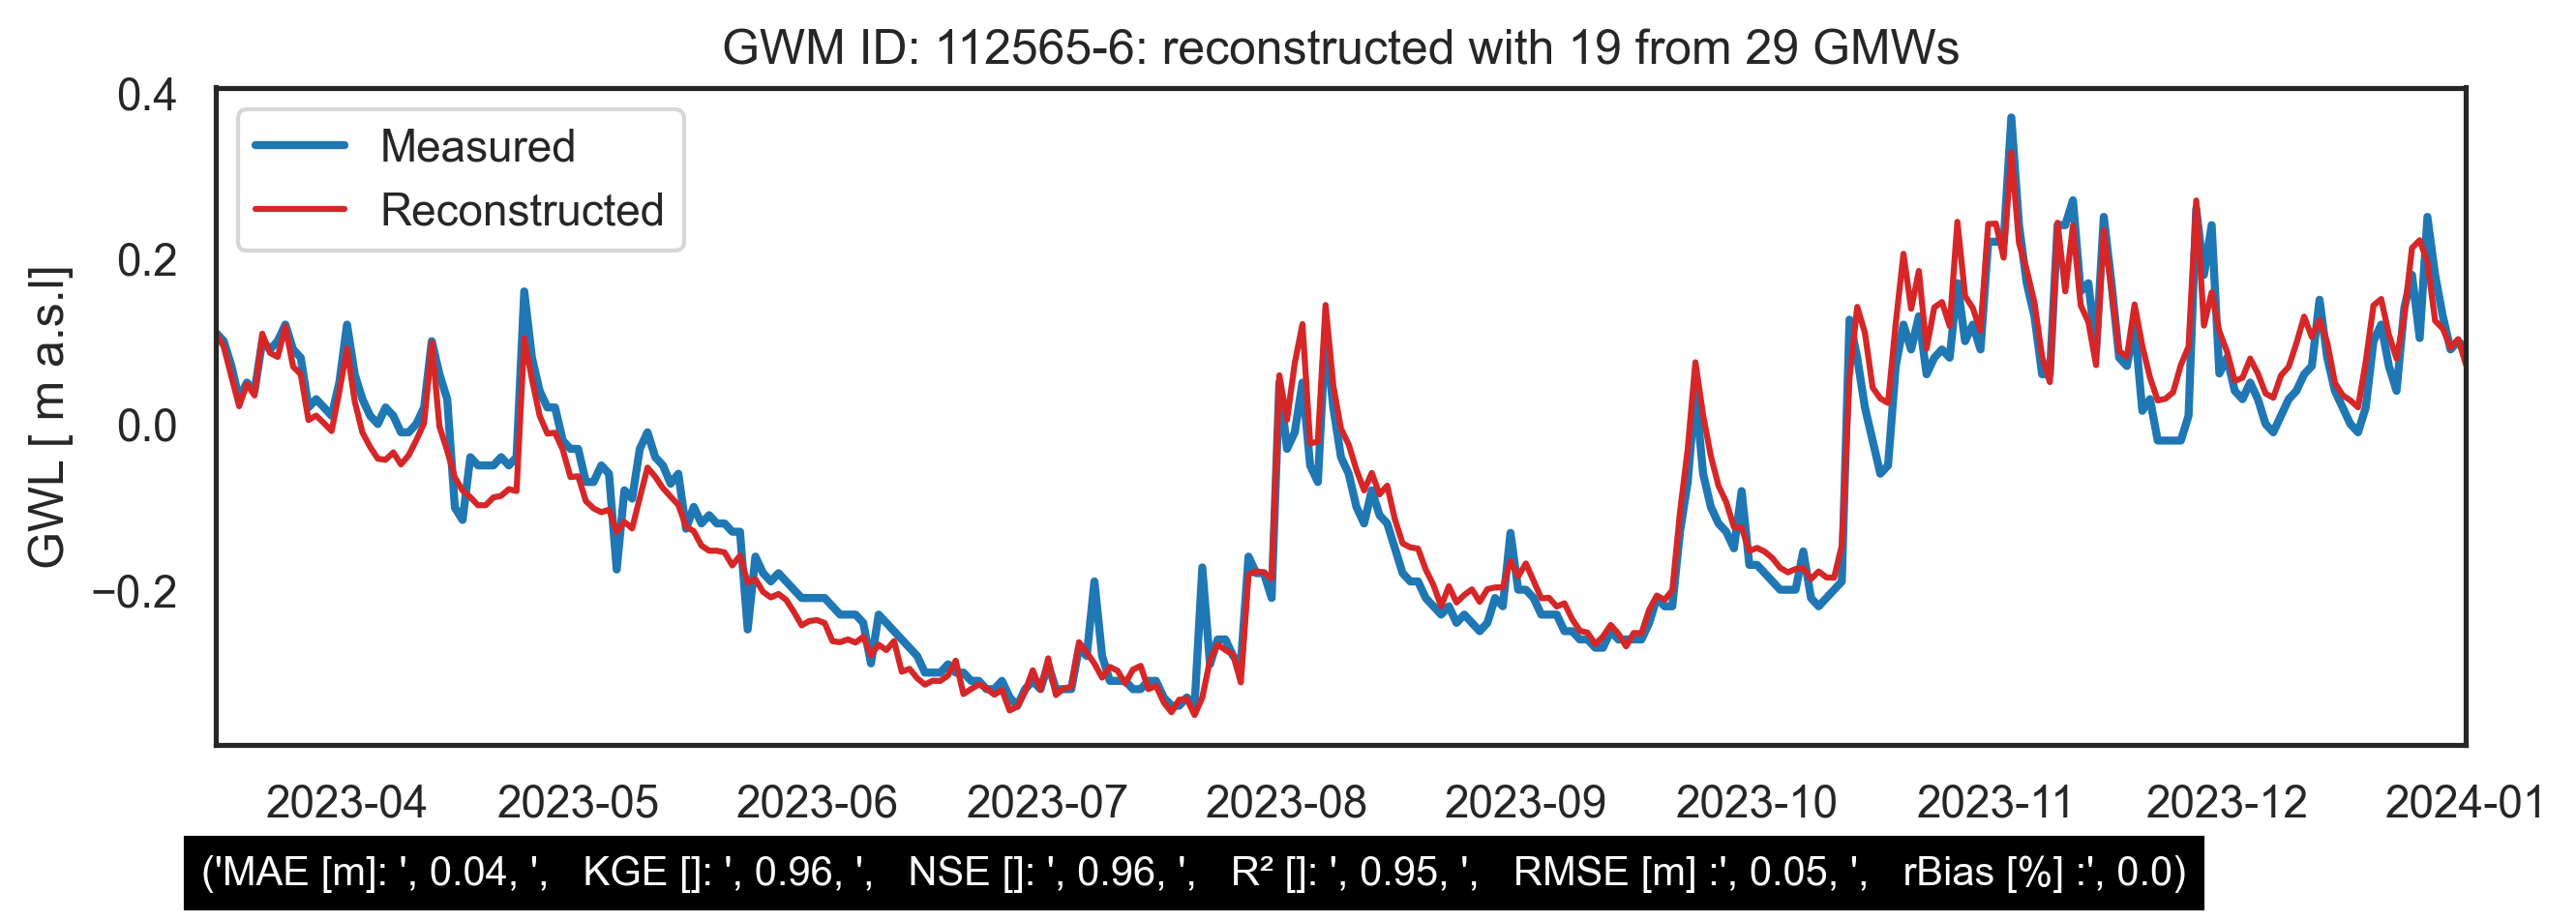
\includegraphics[width=\linewidth]{GWM_reconstructed112565-6.png}
        \caption{Monitoring well: 112565-6.}
        \label{fig:gwm-112565-6}
    \end{minipage}\hfill
    \begin{minipage}{0.48\textwidth}
        \centering
        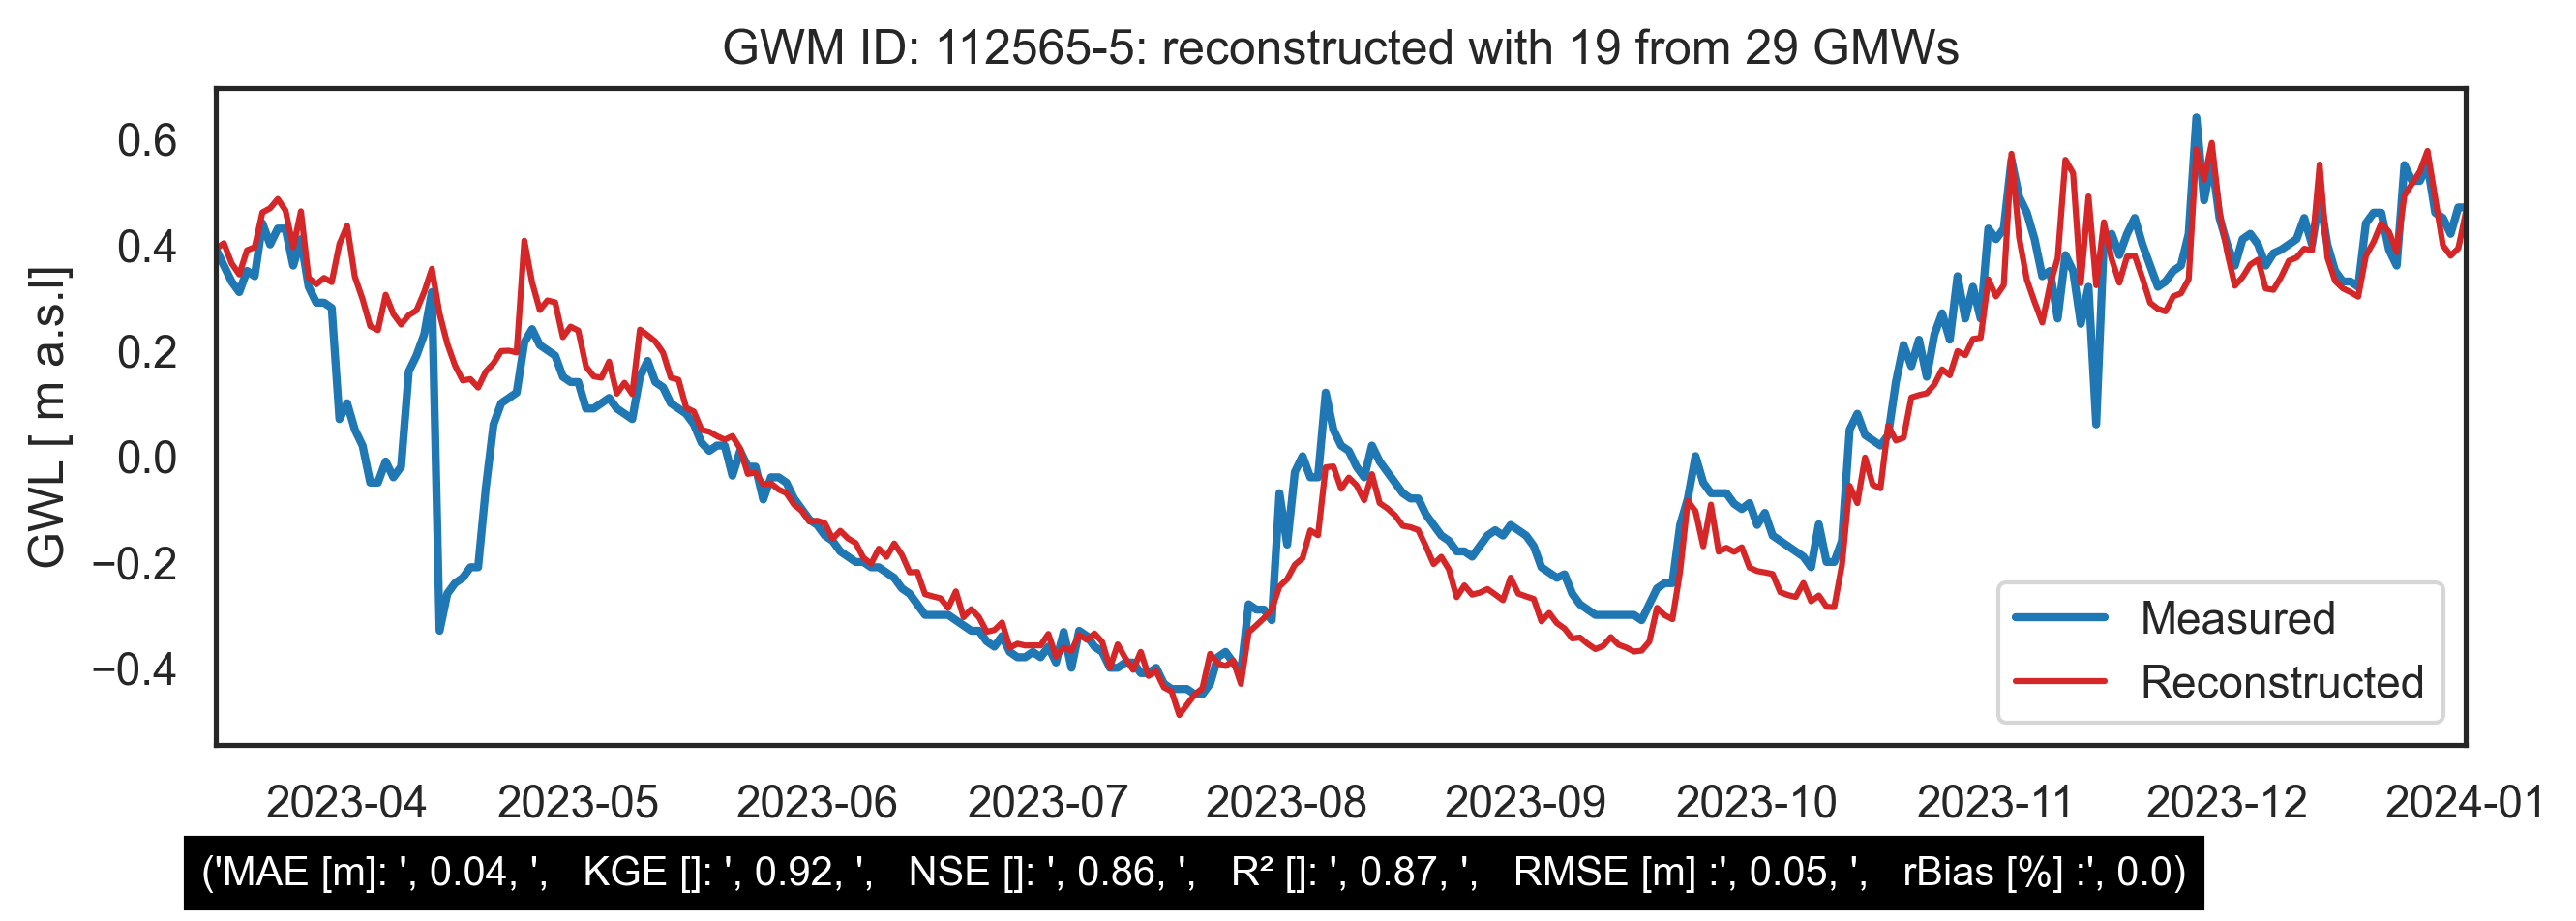
\includegraphics[width=\linewidth]{GWM_reconstructed112565-5.png}
        \caption{Monitoring well: 112565-5.}
        \label{fig:gwm-112565-5}
    \end{minipage}
\end{figure}

As can be seen from the figures, the plots have a comparable plot; a decreasing groundwater level from April 2023 on and reaching the lowest groundwater level in July 2023. In August 2023, the groundwater level increases again to high levels. At the end of August 2023, the groundwater level decreases again, but experiences peak values in October 2023. At the end of 2023, the groundwater levels are increasing again, but at this time of the year, the levels look more constant. 

The measured and reconstructed groundwater levels are tested with the Welch's t-test to determine whether it is the case of a significant difference between the measured and reconstructed groundwater levels. The results are displayed in figure 5.33. Only 4 out of the 10 eliminated monitoring wells experiences a significant difference between the measured and reconstructed groundwater level data. This means that the p-values of the monitoring wells are lower than alpha = 0.05. 

\begin{figure}[htbp]
    \centering
    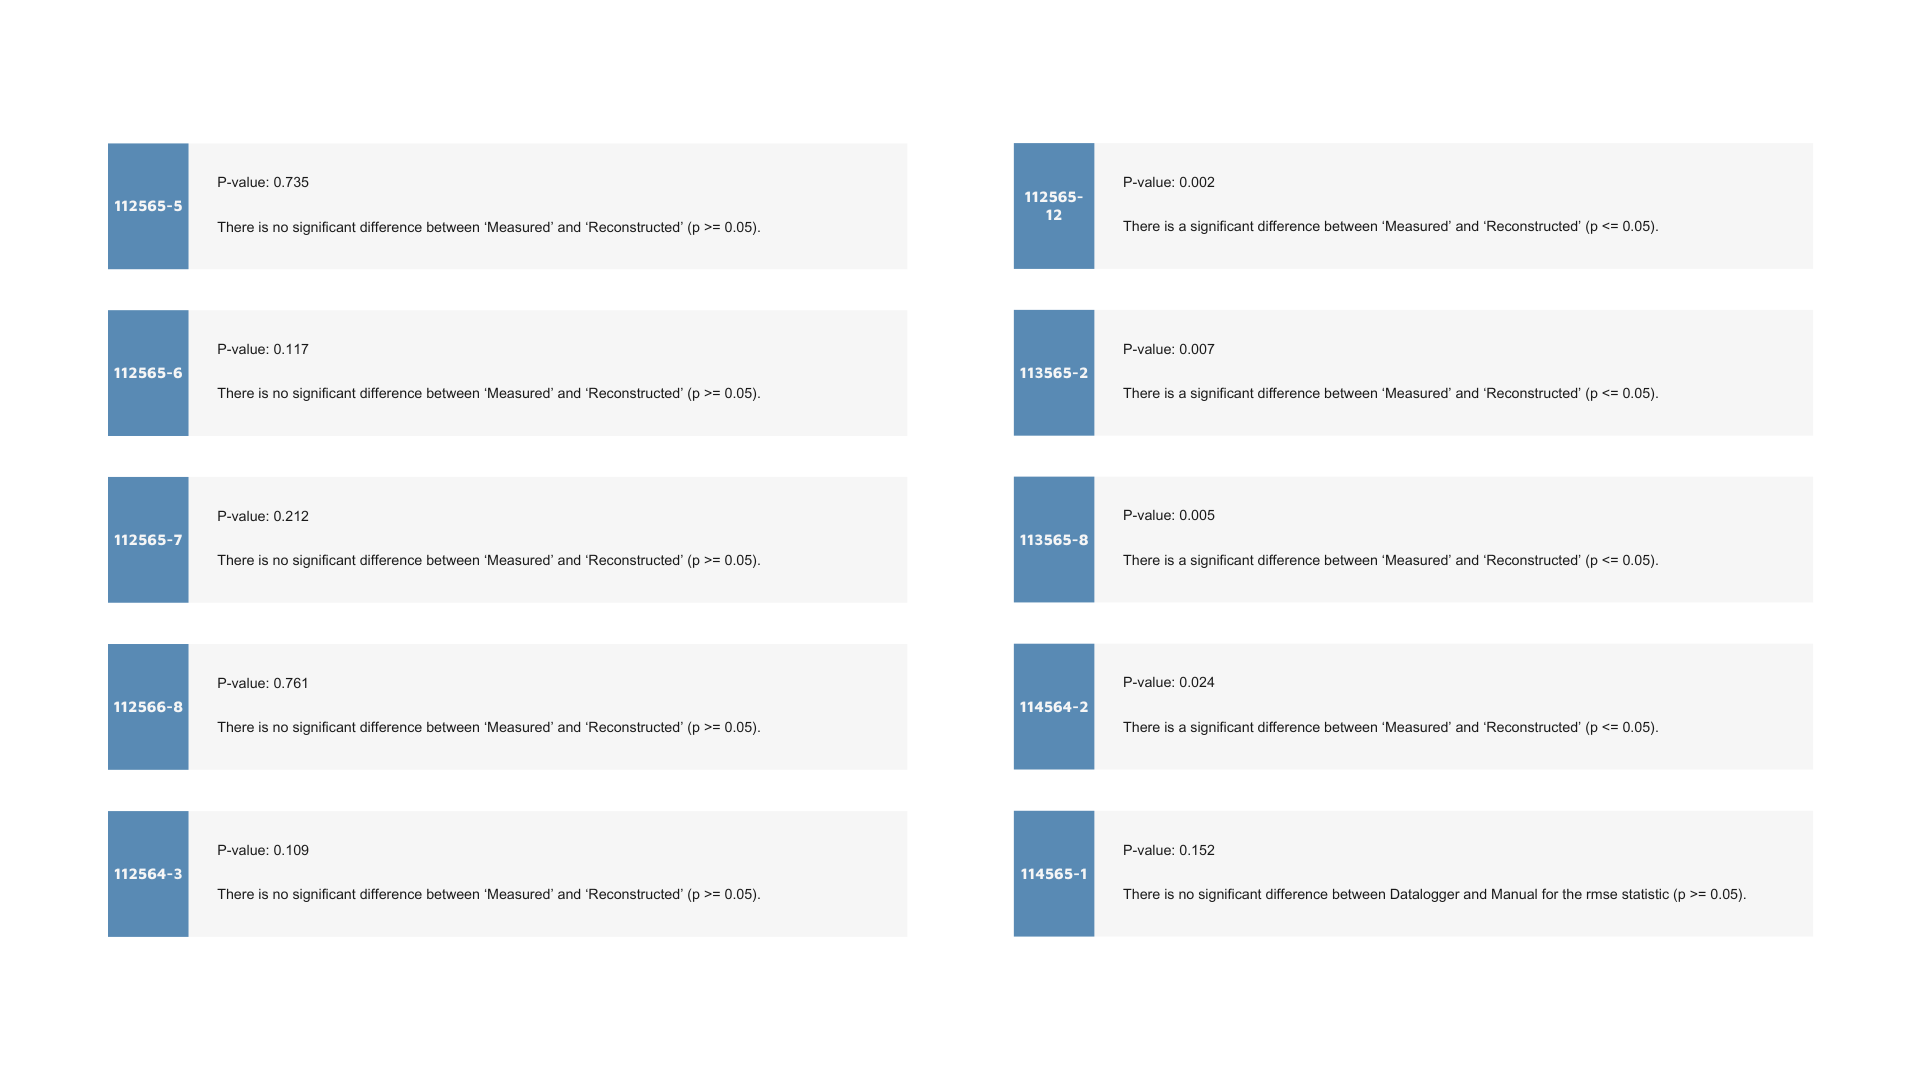
\includegraphics[width=0.80\linewidth]{hydrostatroz.png}
    \caption{Overview of the statistical results of the eliminated monitoring wells. The overview explains the p-value of the monitoring well and whether they experience a significant difference.}
\end{figure}

Additional to the t-test, a Continuous Ranked Probability Score is executed. The CRPS can lay between 0 and 1, where 0 indicates an accurate forecast and 1 indicates an inaccurate forecast. 

\begin{figure}[htbp]
    \centering
    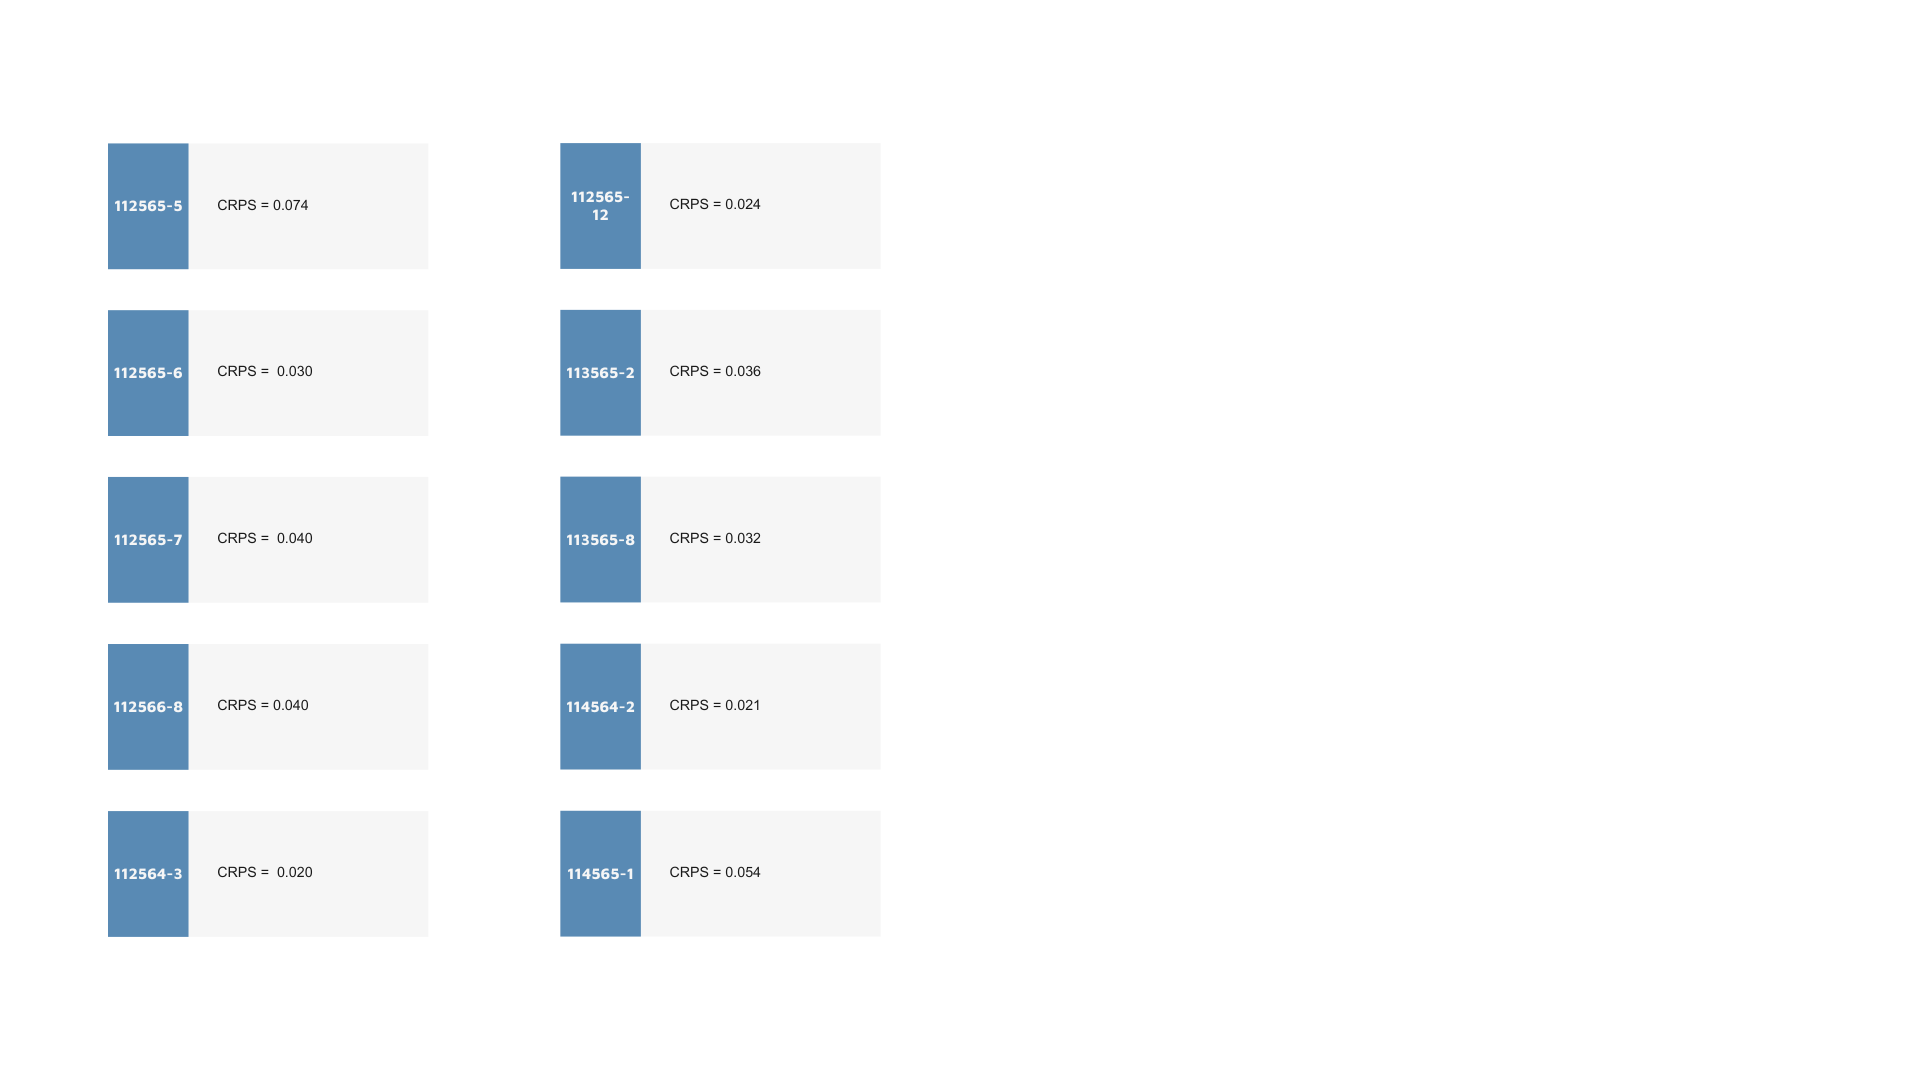
\includegraphics[width=0.80\textwidth]{crpsroz.png}
    \caption{Overview of the CRPS values of the eliminated monitoring wells. The overview explains the CRPS values on a range of 0-1.}
\end{figure}

Based on the overview in figure 5.34, it can be said that monitoring well 112564-3 has the lowest CRPS value and monitoring well 112565-5 has the highest CRPS value. 
\clearpage
Figure 5.35 visualizes a series of boxplots, displaying the distribution of the performance metrics: NSE, R2, and KGE of a network reduction rate of X \%. The orange lines in the boxes explain the median value. The y-axis ranges from 0.825 meters to 1.000 meters. The NSE boxplot has a median value between 0.950 and 0.975 meters. The box itself is a little wider than that, between 0.9480 and 0.980 meters. The whiskers have an equal length and range to 0.9300 at the bottom up to 1.000 meters at the top. There is an outlier present around 0.855 meters, this is indicated by the circle. The R2 boxplot has a similar median value as the NSE boxplot; between 0.950 and 0.975 meters. In comparison with the NSE boxplot the box is a lot smaller, the range of values within this metric is smaller. The whiskers at the bottom and top of the box do not have equal lengths. The whisker at the bottom reaches the same value as the NSE boxplot; 0.9300 meters, while the whisker at the top only reaches a value of 0.975 meters. An outlier is spotted, reaching a value close to 0.875 meters. The KGE boxplot has a much bigger box than the NSE and R2 boxplots, but the median value is also much lower; 0.925 meters. The whisker at the bottom reaches a value up to 0.825 meters, the lowest value a whisker reaches of these three boxplots. The upper whisker, however, is very small and only reaches a value between 0.950 and 0.975 meters. 

\begin{figure}[htbp]
    \centering
    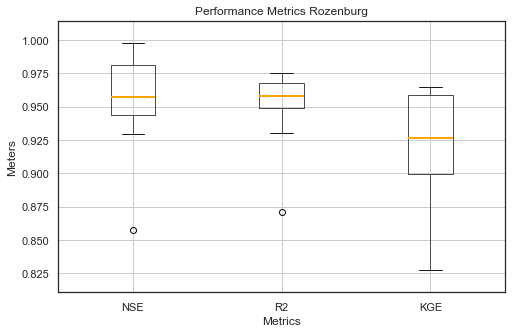
\includegraphics[width=0.80\linewidth]{boxroz.png}
    \caption{Plot with 3 boxplots of performance metrics NSE, R2, and KGE. The orange line indicates the median value. The y-axis ranges from 0.825 to 1.000 meters.}
\end{figure}

\subsubsection{Mean Absolute Error of Reduction}
Based on the reduction percentage of 32\%, reconstruction hydrographs could be plotted in figures 5.23-5.32. The extent to which the reconstructed groundwater level data corresponds to the actual observed data can be determined by the mean absolute error [meters]. The mean absolute error is calculated for every, eliminated monitoring well. A color rank is visualized in figure 5.36 with the level of the calculated mean absolute error (epsg=28992). Blue indicates a low MAE, while yellow indicates a high MAE. The visualization enables the identification of monitoring wells with higher or lower predictive accuracy, which could influence decision-making regarding the placement of future monitoring wells or the scope of maintenance efforts on existing wells. The MAE measures indirectly the performance of the monitoring well regarding data reconstruction. A high MAE in a network of lower MAE values can suggest a vulnerable monitoring well for external, environmental factors. Monitoring wells with a high MAE address the reliability of the data. The monitoring well that is marked with a yellow color indicates a higher MAE value compared to the other monitoring wells. 

\begin{figure}[htbp]
    \centering
    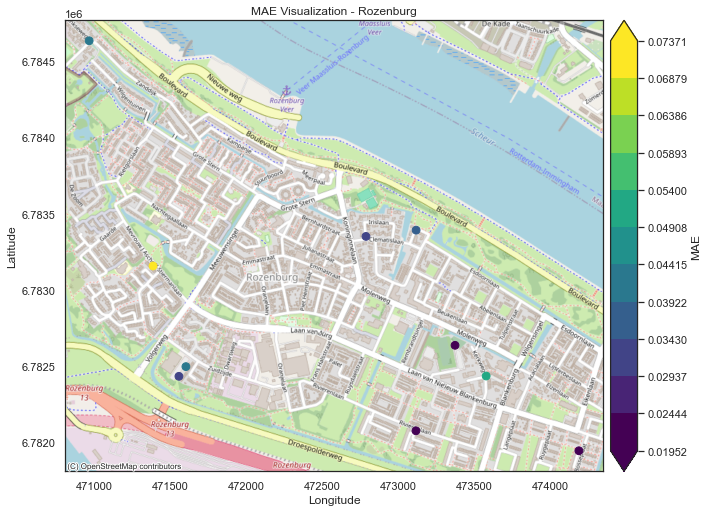
\includegraphics[width=1\linewidth]{mae32roz.png}
    \caption{Geographical representation of the MAE [meters] of every eliminated monitoring well in the neighborhood Rozenburg. The MAE color rank ranges between 0.019 and 0.073 meters.}
\end{figure}

\clearpage

\section{Heijplaat}
\subsection{QGIS and PROWAT}

A multi-colored scatter plot is represented, showing the groundwater level [m MSL] over time [days] for the neighborhood "Heijplaat" in figure 5.37..The x-axis is broad, ranging from 1980 to 2024. Heijplaat has much historical groundwater data available. Each colored dot represents an individual data point from a unique monitoring well, see legend on the right side of the figure. A wide array of groundwater levels is depicted, ranging from below +1.0 to little points of +3.5 m MSL. 
\\
\\
The plot visualizes variation in groundwater levels between different monitoring wells. Some of the monitoring wells perform more stable groundwater levels, while other monitoring wells have an abundant fluctuation. Dense clustering of data points suggests that measurements were taken frequently over that period of time. The variety of colors that are connected to the individual monitoring wells allows the possibility for a comparison of groundwater level trends between monitoring locations within the neighborhood. \\
\begin{figure}[htbp]
    \centering
    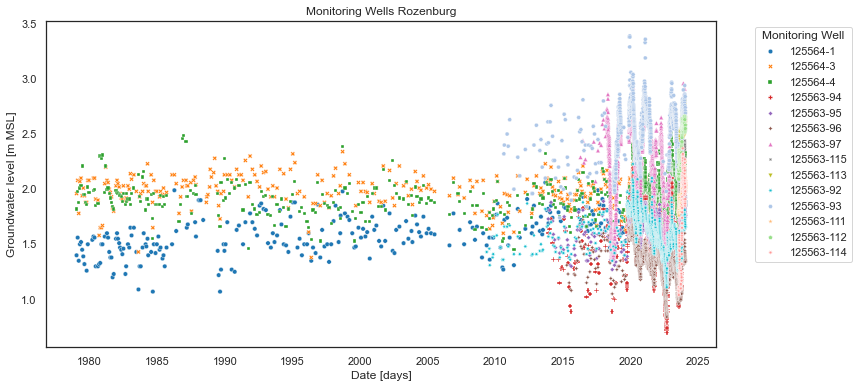
\includegraphics[width=0.75\linewidth]{scatterheij.png}
    \caption{Overview of observed data by manual measurements and data loggers for all 14 monitoring wells in Heijplaat.}
\end{figure}\\

\subsection{Pastas time series modeling}
Similarly to the plot in the section "Rozenburg", the bar plot displays the recharge rates in m/day over a period from 2010 to 2024, figure 5.38. The y-axis quantifies the recharge rate, with values ranging from 0 to 0.07 m/day. The bars show variability in recharge rates over time, where some years experience peaks in recharge (higher recharge rates), which can be due to increased precipitation. As can be seen from the figure, the data is dense, indicating frequent measurements. The pattern of the bars reflect seasonal changes. Lower values of recharge are more frequently observed than high outliers, possibly indicating a baseline level of recharge over the years. Two additional figures of the precipitation and potential evaporation are visualized as well. The data of these figures is combined to determine the recharge rate in the municipal area. 

\begin{figure}[htbp]
    \centering
    \includegraphics[width=0.75\linewidth]{figures/res heij/Recharge Rdam.png}
    \caption{Recharge [m/day] over a period of 2010-2024. Recharge is based on the variables precipitation minus evaporation. Variables are  measured by KNMI at weather station 344 in Rotterdam, The Netherlands.}
\end{figure} 

\begin{figure}[h]
    \centering
    % First figure
    \begin{minipage}{0.45\textwidth}
        \centering
        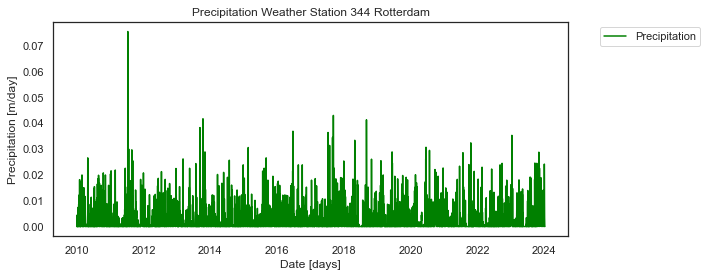
\includegraphics[width=\linewidth]{figures/roz/p.png}
        \caption{Precipitation [m/day] over a period of 2010-2024. Values measured by KNMI at weather station 344 in Rotterdam, The Netherlands.}
        \label{fig:fig1}
    \end{minipage}\hfill
    % Second figure
    \begin{minipage}{0.45\textwidth}
        \centering
        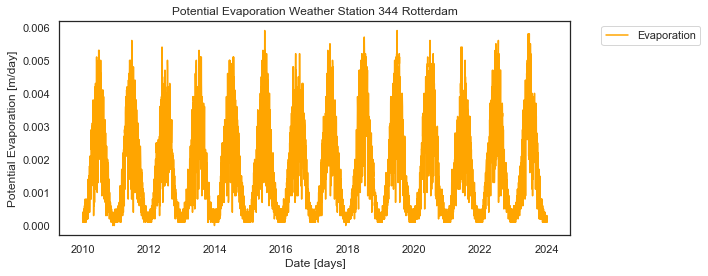
\includegraphics[width=\linewidth]{figures/roz/potevap.png}
        \caption{Potential evaporation [m/day] over a period of 2010-2024. Values measured by KNMI at weather station 344 in Rotterdam, The Netherlands.}
        \label{fig:fig2}
    \end{minipage}
\end{figure}

\newline

\subsubsection{Reverse forecasting}
A part of the Pastas package is reverse forecasting or also called backcasting of the observed data. Reversed forecasting takes place for all the unique monitoring wells present in the case study area. For every monitoring well, three figures are created: 1) Reversed backcasting for data loggers; 2) Reversed backcasting for manual measurements; 3) A combination figure of the first 2 figures combined, see figures 5.41-5.43. 

\begin{figure}[htbp]
    \centering
    % First figure
    \begin{minipage}{0.32\textwidth}
        \centering
        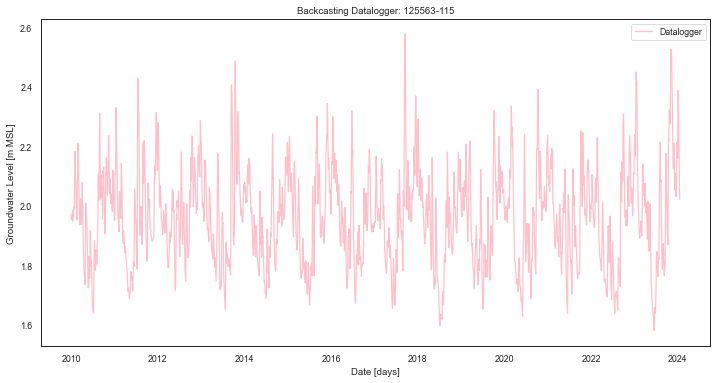
\includegraphics[width=\linewidth]{figures/res heij/dl1125663115.png}
        \caption{Heijplaat 125563-115.}
        \label{fig:fig1}
    \end{minipage}
    \hfill
    % Second figure
    \begin{minipage}{0.32\textwidth}
        \centering
        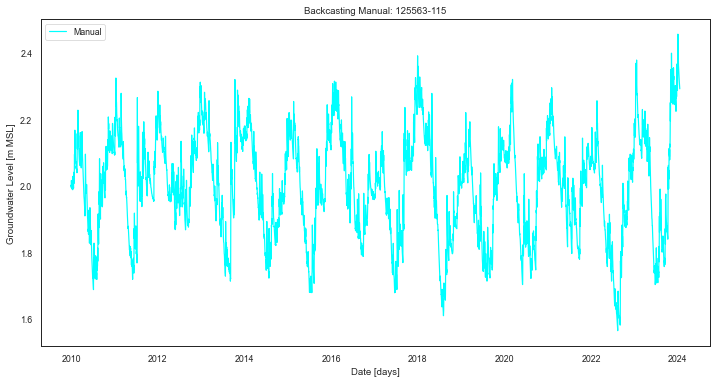
\includegraphics[width=\linewidth]{figures/res heij/hp125563115.png}
        \caption{Heijplaat 125563-115.}
        \label{fig:fig2}
    \end{minipage}
    \hfill
    % Third figure 
    \begin{minipage}{0.32\textwidth}
        \centering
        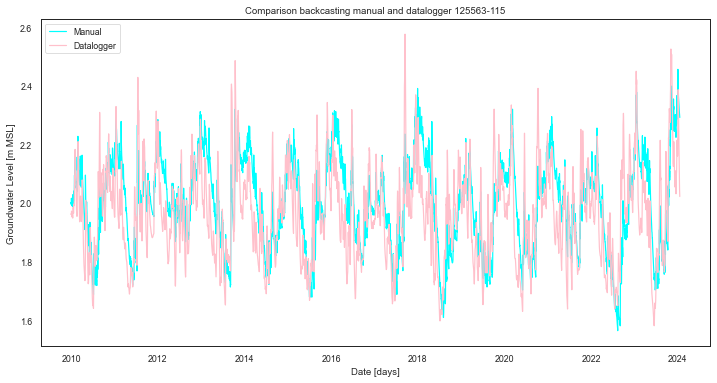
\includegraphics[width=\linewidth]{figures/res heij/comb125563115.png}
        \caption{Heijplaat 125563-115.}
        \label{fig:fig3}
    \end{minipage}
\end{figure}

\clearpage
\subsubsection{Performance metrics}
The barplots shows the performance metrics RMSE, R2, and EVP for all unique monitoring wells with a comparison to a distinction in dataloggers and manual collection method. The first bar plot shows the distribution of RMSE and R2 for every unique monitoring well with a distinction between dataloggers and manual collection. The second bar plot shows the distribution of RMSE and R2 for every unique monitoring well only. The third barplot describes the EVP for every monitoring well with a distinction between the manual collection method and datalogger. Generally, low values of the RMSE indicate a better fit of the model. The R2 values represent the proportion of variance in the observed data that is predictable from the model inputs, with higher values indicating a better fit. Based on the bar plot, the performance of the models for each monitoring well can be compared. Overall, short bars for RMSE (blue and green) and tall bars for R2 (red and orange) indicate a better model performance. An additional bar plot describes the EVP [\%] across the dataset. The EVP is a goodness-of-fit indicator which compares the variance of the observed data and the variance of the residual data (Asmuth von et al., 2012). A low EVP indicates that data could be missing in the data set, where the spatial pattern in the data set could be a possible reason. A statistical test is a follow-up, substantiating the difference between the performance of the two data groups.


\begin{figure}[htbp]
    \centering
    % First figure
    \begin{minipage}{0.48\textwidth}
        \centering
        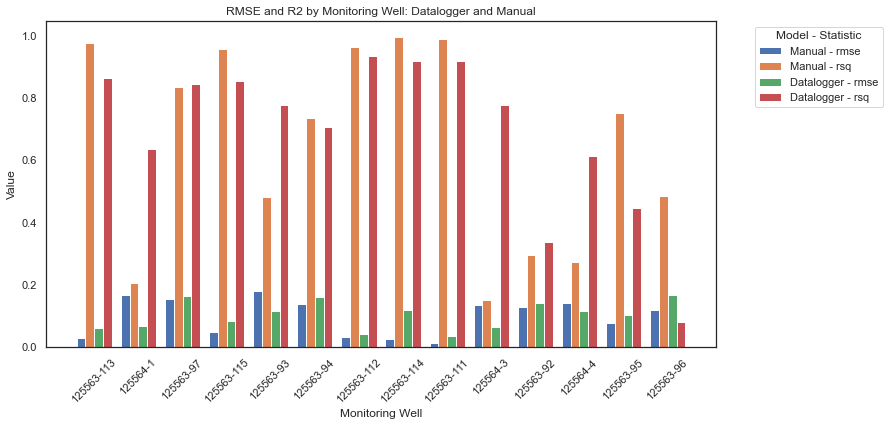
\includegraphics[width=\linewidth]{rmser2heij.png}
        \caption{Bar plot of RMSE and R2 for every monitoring well with a distinction between dataloggers and manual collection.}
        \label{fig:rmser2heij}
    \end{minipage}\hfill
    % Second figure
    \begin{minipage}{0.48\textwidth}
        \centering
        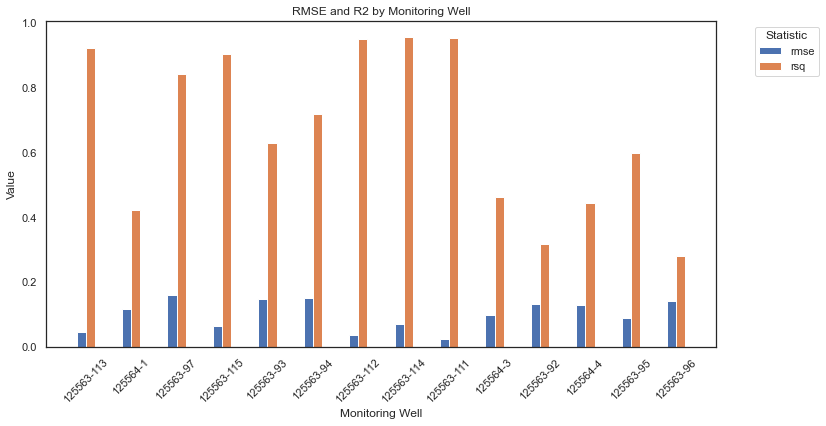
\includegraphics[width=\linewidth]{rmr2heij.png}
        \caption{Bar plot of RMSE and R2 for every monitoring well.}
        \label{fig:rmr2heij}
    \end{minipage}\hfill
    % Third figure
    \begin{minipage}{0.48\textwidth}
        \centering
        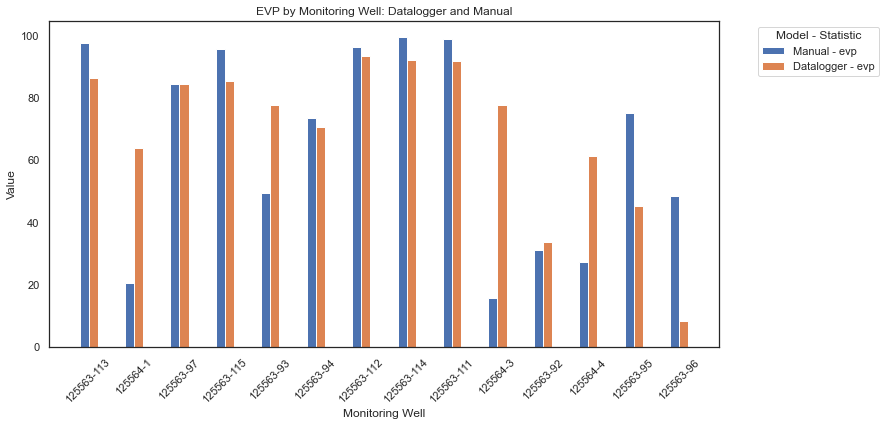
\includegraphics[width=\linewidth]{evpheij.png}
        \caption{Bar plot of EVP for every monitoring well.}   
        \label{fig:evpheij}
    \end{minipage}
\end{figure}

Figure 5.47 displays the result of the Welch's t-test, based on alpha = 0.05. The results of the performance metrics are labeled as RMSE, R2, and EVP. Each performance metric provides the results of the t-statistic and p-value of the Welch's statistical test. The RMSE (blue section), explains that the t-statistic is low and a minimal difference is present between the dataloggers and manual collection method. The p-value is higher than alpha, indicating that the difference is not statistically significant. There is no evidence that one of the data groups provides more accurate measurements. The R2 (orange section) explains that the t-statistic is positive, it is a small t-statistic and shows a difference between the two data groups. The p-value is slightly higher than alpha = 0.05, indicating no significant difference. The last metric is the EVP (green section). The t-statistic of the EVP has a positive value as well as a p-value higher than alpha. The percentage of the total variance in the observed data does not differ between the two data collection methods.

\clearpage

\begin{figure}[htbp]
    \centering
    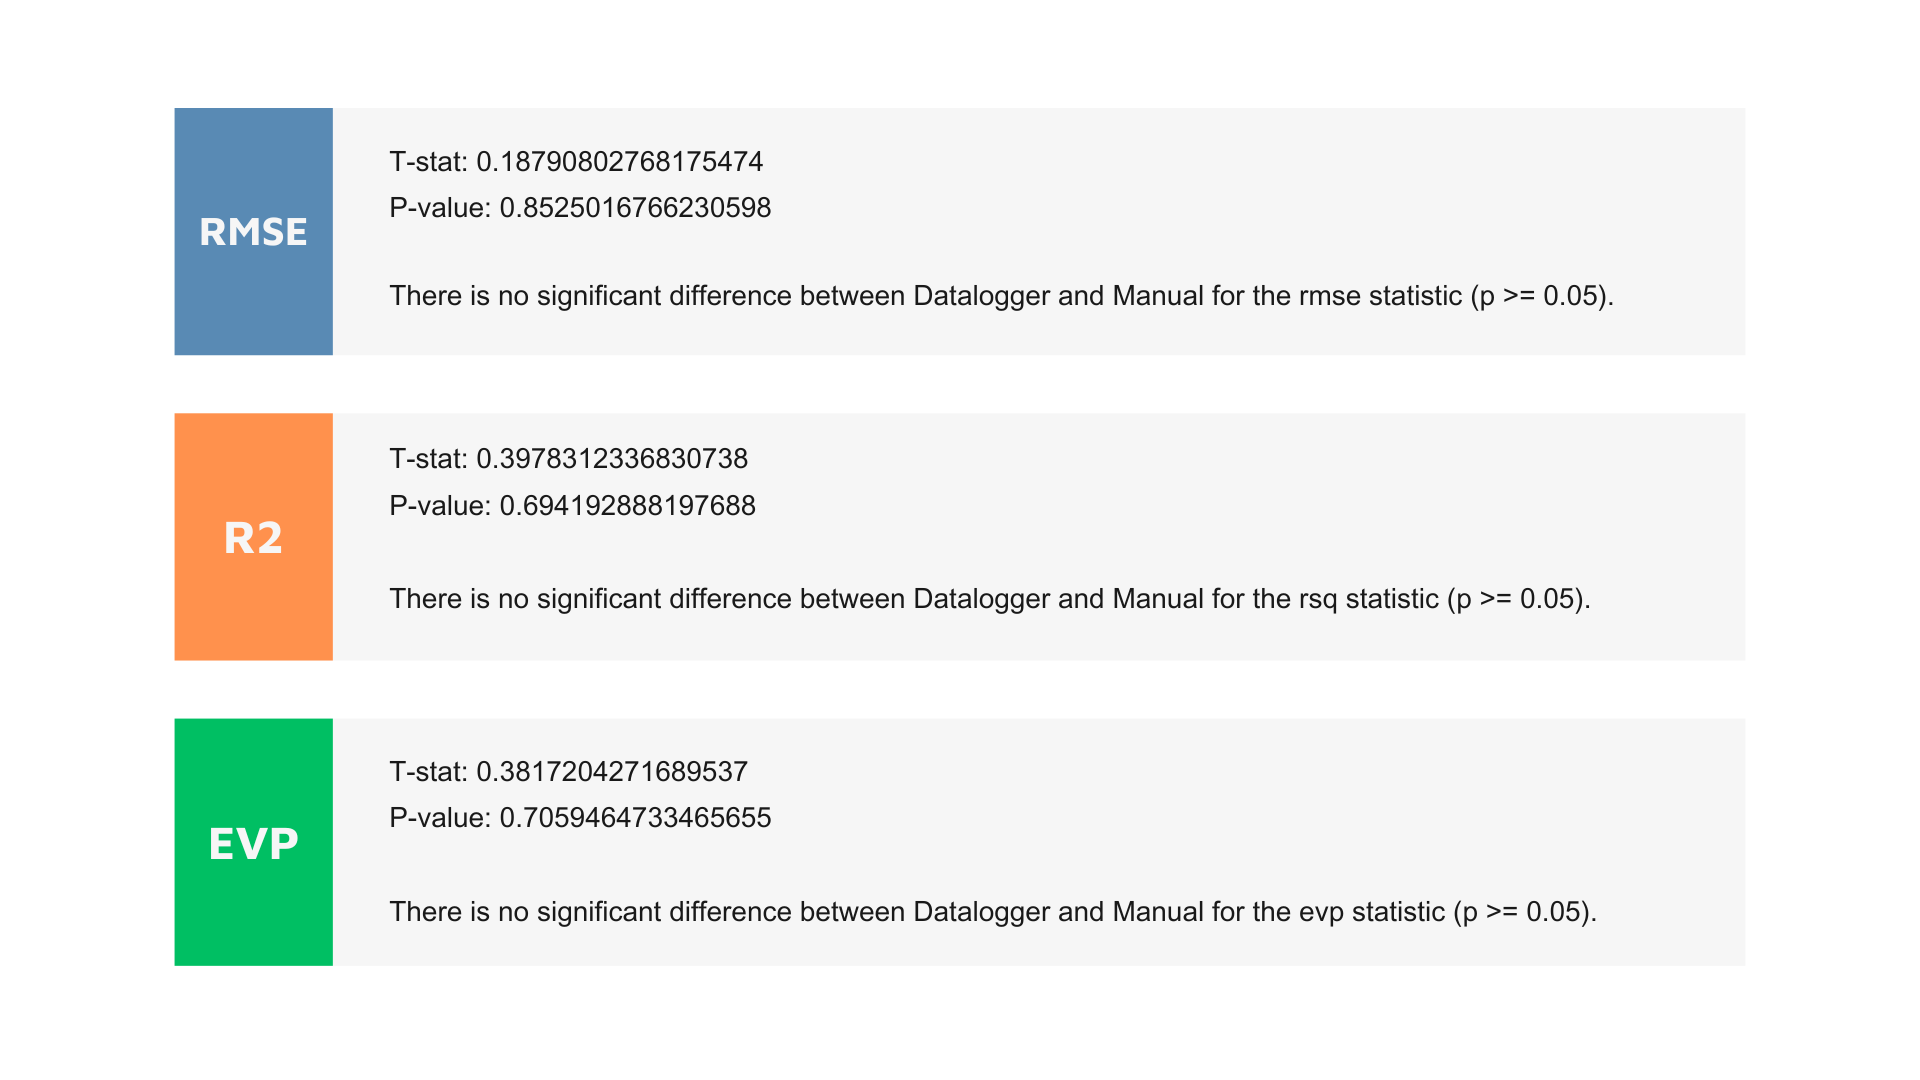
\includegraphics[width=0.80\linewidth]{BARPLOTHEIJ.png}
    \caption{Overview of performance metrics of the statistical Welch's t-test and the difference between dataloggers and manual collection.}   
\end{figure}

According to the Welch's t-test, no substantial discrepancies were found in the data groups. None of the P-values are below the cut-off of alpha = 0.05. Consequently, just like the area "Rozenburg", it was decided to proceed with the group that is specialized in data loggers. Despite statistical significance, other factors are crucial in environmental sciences. Hence, the datalogger group is chosen, merging observed and simulated data into one dataset and excluding the manual measurements.

\subsubsection{Creation of new data frame}
The scatter plot below visualizes the observed data logger with the pink scatter and the simulated data of the data loggger is visualized by the green scatter. On the x-axis the time period [days] is shown and on the y-axis the groundwater level [m MSL]. Figure 5.48 visualizes only monitoring well X, the remaining monitoring wells of the neighborhood are available in the appendix and/or GitHub.


\begin{figure}[htbp]
    \centering
    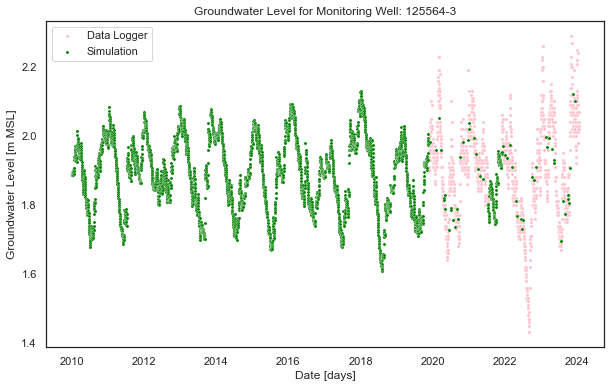
\includegraphics[width=0.80\linewidth]{11255643heij.png}
    \caption{Scatter plot of merged data frames: observed data by dataloggers and simulation data based on datalogger data for monitoring well 1125564-3.}   
\end{figure}


\subsection{QR factorization}
Using QR factorization as foundation, a hierarchical list of the monitoring wells in Heijplaat is created. The optimal reduction percentage is determined and reduction tests can be executed. Resulting in an overview of eliminated monitoring wells and their capability to reconstruct future groundwater levels in the network.

\subsubsection{1D hydrograph data}
Figure 5.49 is a geographical representation (epsg=28992) visualizing the spatial distribution of monitoring wells in the neighborhood "Heijplaat", plotted on a x,y coordinate system. Within the map, a scatter plot with a color scale represents the groundwater level measurements taken at the monitoring wells. The color scale has a range between -0.5 m to +2.0 m MSL. Each monitoring well represents a location as well as the color of monitoring well represents the value on the color scale. In the northwest of the neighborhood, the groundwater level seems to be higher than the groundwater level in the south of the neighborhood.

\begin{figure}[htbp]
    \centering
    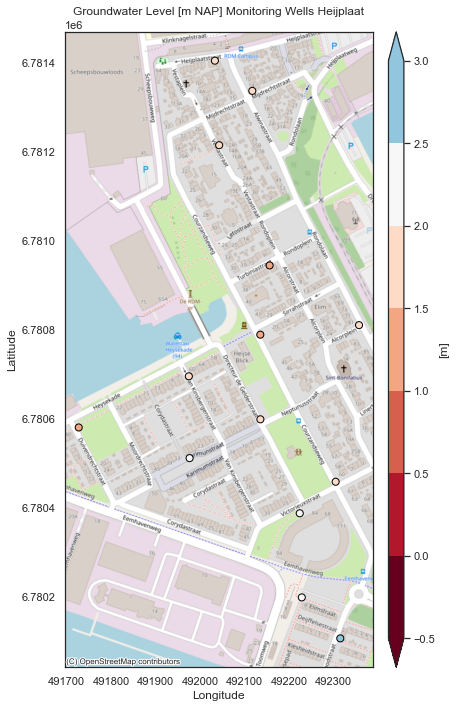
\includegraphics[width=0.60\linewidth]{gwlheij.png}
    \caption{Groundwater level [m MSL] visualized in a geographical map with a color rank that describes the groundwater level observed in 14 monitoring wells of Heijplaat.}   
\end{figure}

\clearpage

\subsubsection{Sampling data}
Preprocessing of the data includes transforming the data frame into an array, implementing both global and local centering methods, and splitting the dataset into an 80/20 ratio training and test set distribution. The result of the preprocessing is as follows, see table 5.2.

\begin{table}[htbp]
\centering
\caption{Summary of sampling data.}
\label{tab:sampling_data}
\begin{tabular}{|l|l|}
\hline
\textbf{Parameter}                           & \textbf{Value}                                \\ \hline
Sampling period                              & 2020-01-02 00:00:00 to 2024-01-01 00:00:00   \\ \hline
Number of samples                            & 1462                                          \\ \hline
Number of features (sensors)                 & 14                                            \\ \hline
Shape of X (samples, sensors)                & (1462, 14)                                    \\ \hline
Min. and max. value                          & 0.7 [m]; 3.36 [m] \\ \hline
Min. and max. centered value                 & -0.768 [m] 0.589 [m]                         \\ \hline
Min. and max. centered value (exact)         & -0.7679038683451884 [m]; 0.5894112429907086 [m] \\ \hline
Mean centered data                           & 0.0 [m]                                     \\ \hline
Train data, Test data                        & 1169 , 293                                   \\ \hline
Train data, Test data (percentage)           & 80\%, 20\%                                  \\ \hline
\end{tabular}
\end{table} 

\subsubsection{Hierarchy of monitoring wells}
Figure 5.50 is a geographical representation (epsg=28992) of data points plotted on a x,y coordinate system. The horizontal axis is labeled as longitude and the vertical axis is labeled as latitude. The data points are scattered across the study area within a polygonal boundary that represents the neighborhood "Heijplaat". Each monitoring well monitoring well is color-coded according to the color bar on the right side of the plot. The color indicates the rank of each monitoring well. The color bar has a range between dark blue for the lowest values (0) to yellow for the highest values (14). The distribution of the color code does not follow a clear pattern within the study area. Some clusters of higher or lower ranked monitoring wells are present. Overall, the monitoring wells with additional value are marked blue. They show possibly show flashiness in their data, meaning a high frequency and rapidity in short term changes with strong irregular patterns. According to Ohmer et al. (2022), these monitoring wells indicate strong interaction with surface waters and boundary inflows. As well as a high seasonality and low variability. The monitoring wells that likely do not have additional value to the network are marked yellow. These wells show low flashiness and high seasonality. A cluster of redundant monitoring wells appears to be located at the southern side of the neighborhood. The data cluster could indicate a region of low data variability and flashiness. Towards the north of the neighborhood, a higher rank is also noted. 

\begin{figure}
    \centering
    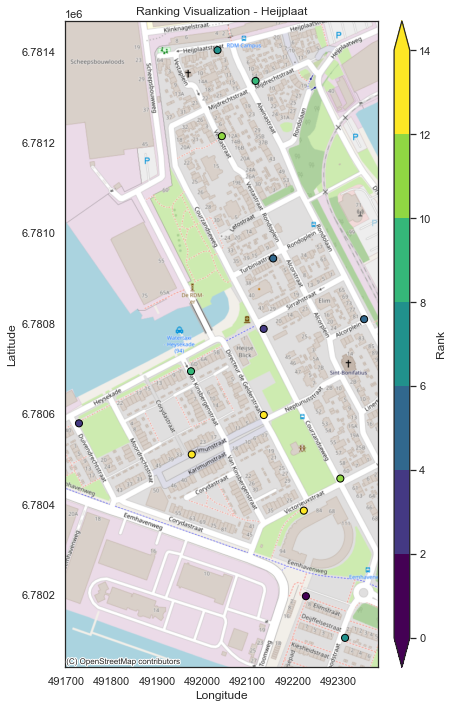
\includegraphics[width=0.80\linewidth]{rankheij.png}
    \caption{Geographical map visualizing the calculated ranking of all monitoring wells in the neighborhood Heijplaat.}    
\end{figure}

\clearpage

\subsubsection{Determining the optimal reduction rate}
Figures 5.51-5.54 visualize the Reconstruction Error of Heijplaat, plotting the root mean square error (RMSE) in meters on the y-axis against the number of monitoring wells on the x-axis. The line graph shows a decreasing trend in the RMSE as the number of monitoring wells increasing, suggesting that more monitoring wells contribute to a lower reconstruction error in the data. In the figures, the orange marked point marks the optimal number of monitoring wells where the reconstruction error reaches the threshold that is indicated by the orange line. The threshold is an acceptable level of RMSE for the reconstruction process. The original groundwater monitoring network of Heijplaat includes 14 monitoring wells. 
\newline
In figure 5.51, a reduction of 25\% explains that a number of 10 monitoring wells is the most optimal with a removal of 4 monitoring wells. The RMSE is calculated to determine the optimal number of monitoring wells in the neighborhood. Figure 5.52, demonstrates a trend, based on a reduction rate of 50 \%. The RMSE decreases as more monitoring wells are added to the network. At the point of n = 7 on the x-axis, an orange dot is indicated. Beyond this point, the decrease in RMSE slows down, suggesting returns on error reduction after a specific number of monitoring wells is reached. 

\begin{figure}[htbp]
    \centering
    \begin{minipage}{0.45\linewidth}
        \includegraphics[width=\linewidth]{25heij.png}
        \caption{Reconstruction error calculated for the neighborhood with a network reduction of 25\%. With a reduction rate of 25\%, 4 wells are eliminated while 10 wells remain.}
        \label{fig:first-figure}
    \end{minipage}
    \hfill
    \begin{minipage}{0.45\linewidth}
        \includegraphics[width=\linewidth]{50heij.png}
        \caption{Reconstruction error calculated for the neighborhood with a network reduction of 50\%. With a reduction rate of 50\%, 7 wells are eliminated while 7 wells remain.}
        \label{fig:second-figure}
    \end{minipage}
\end{figure}

Figure 5.53, displays a trend where the RMSE decreases as the number of monitoring wells increases. The RMSE declines as the monitoring well count approach reaches the point above 3 monitoring wells. This is the point marked with the orange dashed line. The line marks the optimal number of monitoring wells where the reconstruction error reaches the threshold value. The threshold value is an acceptable level of RMSE for the reconstruction process. Initially, Heijplaat includes 14 monitoring wells. The results of the RMSE explains that only 3 monitoring wells remain, 11 monitoring wells have to be removed from the local network if a reduction of 75\% is being used in the approach. A reduction rate of 75 \% explains an equilibrium state between the number of monitoring wells and the reconstruction error is achieved. 
\newline
Continuing with figure 5.54, the Reconstruction Error for a reduction of 90\% is displayed. The figure plots the RMSE in meters on the y-axis against the number of monitoring wells on the x-axis. The line graph shows a decreasing trend in the RMSE as the number of monitoring wells increases. The orange marked point marks the optimal number of monitoring wells where the reconstruction error reaches the threshold that is indicated by the orange line. The threshold is the acceptable level of RMSE for the reconstruction process. Heijplaat includes 14 monitoring wells. The results of the reduction rate describes that 1 monitoring well remains, while 13 monitoring wells are eliminated from the network.

\clearpage
\begin{figure}[htbp]
    \centering
    \begin{minipage}{0.45\linewidth}
        \includegraphics[width=\linewidth]{75heij.png}
        \caption{Reconstruction error for the neighborhood with a network reduction of 75\%. With a reduction rate of 75\%, 11 wells are eliminated while 3 wells remain.}
        \label{fig:third-figure}
    \end{minipage}
    \hfill
    \begin{minipage}{0.45\linewidth}
        \includegraphics[width=\linewidth]{90heij.png}
        \caption{Reconstruction error for the neighborhood with a network reduction of 90\%. With a reduction rate of 90\%, 13 wells are eliminated while 1 well remains.}
        \label{fig:fourth-figure}
    \end{minipage}
\end{figure}

Based on sensitivity analysis regarding determining the lowest RMSE and MAE as posisble for the neighborhood, seperate analysis are executed to determine the optimal RMSE and MAE. Further in the analysis, the two performance metrics are combined to determine the lowest RMSE and MAE possible. 

\begin{figure}[h]
    \centering
    \begin{minipage}{0.45\linewidth}
        \includegraphics[width=\linewidth]{heij37rr.png}
        \caption{Optimal reduction percentage of 49\% based on a sensitivity analysis of RMSE.}
    \end{minipage}
    \hfill
    \begin{minipage}{0.45\linewidth}
        \includegraphics[width=\linewidth]{heij37rrrm.png}
        \caption{Optimal reduction percentage of 73\% based on a sensitivity analysis of RMSE.}
    \end{minipage}
\end{figure}

The normalized RMSE and MAE are combined in figure 5.57. The figure acts as a tool to determine the optimal reduction rate for Heijplaat. The optimal reduction rate lies between 30 and 40\%. More specifically, a reduction rate of 37\% is achieved with a combined RMSE and MAE of 0.2983.

\clearpage

\begin{figure}[htbp]
    \centering
    \includegraphics[width=0.70\linewidth]{heijopt.png}
    \caption{Visualization of the normalized RMSE and MAE to determine the optimal reduction rate for the GWMN of Heijplaat. The optimal reduction rate lies between 30 and 40\%.}
\end{figure}


\subsubsection{The optimal reduction rate}
According to the sensitivity analysis of the normalized RMSE and MAE, the optimal reduction rate of a monitoring network consisting of 14 monitoring wells counts up to an optimal reduction rate of 37\%. A reduction rate of 37\% implies that the optimal number of monitoring wells in the neighborhood is 8, meaning that 6 monitoring wells are planned to be eliminated, see figure 5.58. 
\begin{figure}[htbp]
    \centering
    \includegraphics[width=0.70\linewidth]{37heij.png}
    \caption{Reconstruction error for the neighborhood with a network reduction of 37\%. The blue line shows RMSE variation with the number of monitoring wells, while the orange dashed lane indicates the optimal well count for the lowest RMSE. With a reduction rate of 37\%, 6 monitoring wells are planned to be eliminated and 8 monitoring wells remain.}
    \label{fig:enter-label}
\end{figure}

The reconstruction capability of the eliminated monitoring wells is tested through the creation of hydrographs. The hydrographs include a measured and reconstructed plot. The measured plot (blue line) marks the observed data measured by Gemeente Rotterdam, while the reconstructed plot (red line) marks the reconstructed data based on the observed data and the goodness-of-fit of the model. Performance metrics (MAE, KGE, NSE, R2, RMSE, rBIAS) regarding the goodness-of-fit are available underneath the figure. In figures 5.59-5.64, the hydrographs of the eliminated monitoring wells are shown.
\clearpage


\begin{figure}[h]
    \centering
    % Eerste rij
    \begin{minipage}{0.45\linewidth}
        \includegraphics[width=\linewidth]{GWM_reconstructed125563-111.png}
        \caption{Monitoring well: 125563-111.}
        \label{fig:label1}
    \end{minipage}
    \hfill
    \begin{minipage}{0.45\linewidth}
        \includegraphics[width=\linewidth]{GWM_reconstructed125563-112.png}
        \caption{Monitoring well: 125563-112.}
        \label{fig:label2}
    \end{minipage}
    
    % Tweede rij
    \begin{minipage}{0.45\linewidth}
        \includegraphics[width=\linewidth]{GWM_reconstructed125563-113.png}
        \caption{Monitoring well: 125563-113.}
        \label{fig:label3}
    \end{minipage}
    \hfill
    \begin{minipage}{0.45\linewidth}
        \includegraphics[width=\linewidth]{GWM_reconstructed125563-95.png}
        \caption{Monitoring well: 125563-95.}
        \label{fig:label4}
    \end{minipage}
    
    % Derde rij
    \begin{minipage}{0.45\linewidth}
        \includegraphics[width=\linewidth]{GWM_reconstructed125564-1.png}
        \caption{Monitoring well: 125564-1.}
        \label{fig:label5}
    \end{minipage}
    \hfill
    \begin{minipage}{0.45\linewidth}
        \includegraphics[width=\linewidth]{GWM_reconstructed125564-3.png}
        \caption{125564-3.}
        \label{fig:label6}
    \end{minipage}
\end{figure}
As can be seen from the figures, the plots have comparable trends; a decreasing groundwater level from April to July 2023. An increase occurs in July towards mid August 2023. During the start of Fall, a small increase in groundwater level occurs in October with strong increases in November and December 2023. In January 2024, the groundwater level is just as high as at the beginning of November 2023. 
\newline
\newline
The measured and reconstructed groundwater levels are tested with the Welch's t-test to determine whether it is the case of a significant difference between the measured and reconstructed groundwater levels. The results are displayed in figure 5.65.  5 out of 6 eliminated monitoring wells experience a significant difference between the measured and reconstructed groundwater level data. This means that the p-values of the monitoring wells are lower than alpha = 0.05.

\begin{figure}[htbp]
    \centering
    \includegraphics[width=0.70\linewidth]{T-TEST hij.png}
    \caption{Overview of the statistical results of the eliminated monitoring wells. The overview explains the p-value of the monitoring wells and whether they experience a significant difference.}
    \label{fig:enter-label}
\end{figure}

\clearpage
Additional to the t-test, a Continuous Ranked Probability Score is executed. The CRPS can lay between 0 and 1, where 0 indicates an accurate forecast and 1 indicates an inaccurate forecast.

\begin{figure}[htbp]
    \centering
    \includegraphics[width=0.70\linewidth]{crpsheij.png}
    \caption{Overview of the CRPS values of the eliminated monitoring wells. The overview explains the CRPS values on a range of 0-1.}
    \label{fig:enter-label}
\end{figure}

Based on the overview in figure 5.66, it can be said that monitoring well X has the lowest CRPS value and monitoring well X has the highest CRPS value. 
\newline
\newline
Figure 5.67 visualizes a series of boxplots, displaying the distribution of the performance metrics: NSE, R2, and KGE of a network reduction rate of X \%. The orange lines in the boxes explain the median value. The y-axis ranges from X to X meters. The NSE has a median value between X and X meters. 



\begin{figure}[htbp]
    \centering
    \includegraphics[width=0.45\linewidth]{boxheij.png}
    \caption{Plot with 3 boxplots of performance metrics NSE, R2, and KGE. The orange line indicates the median value. The y-axis ranges from 0.7 to 1.0 meters}
\end{figure}


\clearpage
\subsubsection{Mean Absolute Error of Reduction}
Based on the reduction percentage of 37\%, reconstruction hydrographs could be plotted in figures 5.59-5.64. The extent to which the reconstructed groundwater level data corresponds to the actual observed data can be determined by the mean absolute error [meters]. The mean absolute error is calculated for every, eliminated monitoring well. A color rank visualizes the level of the calculated mean absolute error (epsg=28992) in figure 5.68. Blue indicates a low MAE, while yellow indicates a high MAE. The visualization enables the identification of monitoring wells with higher or lower predictive accuracy, which could influence decision-making regarding the placement of future monitoring wells or the scope of maintenance efforts on existing wells. The MAE measures indirectly the performance of monitoring wells regarding data reconstruction. A high MAE in a network of lower MAE values can suggest a vulnerable monitoring well for external, environmental factors. Monitoring wells with a high MAE address the reliability of data. The monitoring well that is marked with a yellow color indicates a higher MAE value compared to the other monitoring wells. 

\begin{figure}[htbp]
    \centering
    \includegraphics[width=0.50\linewidth]{37maeheij.png}
    \caption{Geographical representation of the MAE [meters] of every eliminated monitoring well in the neighborhood Rozenburg. The MAE color rank ranges between -0.20 and 0.10 meters.}
    \label{fig:enter-label}
\end{figure}
\clearpage
